\documentclass[12pt,a4paper,titlepage,xcolor=dvipsnames,bibliography=totoc, listof=totoc]{scrartcl}
%%%%%%%%%%%%%%%%%%%%%%%%%%%%%%%%%%%%%%%%%%%%%%%%%%%%%%%%%%%%%%%%%
\label{Preamble}			%	Preamble
%%%%%%%%%%%%%%%%%%%%%%%%%%%%%%%%%%%%%%%%%%%%%%%%%%%%%%%%%%%%%%%%%
%	Packages:		form/packages
%%%%%%%%%%%%%%%%%%%%%%%%%%%%%%%%%%%%%%%%%%%%%%%%%%%%%%%%%%%%%%%%%
\label{Packages}	%	Packages
%%%%%%%%%%%%%%%%%%%%%%%%%%%%%%%%%%%%%%%%%%%%%%%%%%%%%%%%%%%%%%%%%
%	Font / Script
\RequirePackage[utf8]{inputenc} 		%	Umlaute
\RequirePackage[T1]{fontenc}			%	Standardschrift, Trennung
\RequirePackage{xspace}					%	Leerzeichen
\RequirePackage{pifont}
\RequirePackage{kpfonts}
\RequirePackage{calligra}
\RequirePackage[ngerman]{babel}
\RequirePackage{ifthen}
\RequirePackage[table]{xcolor}
\RequirePackage{pdflscape}
\RequirePackage{afterpage}
\RequirePackage{capt-of}
\RequirePackage{float}
\RequirePackage{bbm}
\RequirePackage{dashrule}
\RequirePackage{url}

%-------------------------------------------------------------
%	Math
\RequirePackage{amssymb,amsmath, amsthm}		%	Math Mode Enhancement
\RequirePackage{array}
\RequirePackage{marvosym}				%	Euro Symbol and others
\RequirePackage{multicol}
\RequirePackage[linesnumbered,ruled,vlined,noend]{algorithm2e}
\SetKwIF{If}{ElseIf}{Else}{if}{:}{else if}{else:}{end if}%
\SetKwFor{While}{while}{:}{end while}%
\SetKwFor{For}{for}{:}{end for}
\SetKwRepeat{Do}{do}{while}
\SetKw{KwGoTo}{go to}

\RequirePackage{thmtools}
\RequirePackage{smartdiagram}
\RequirePackage{listings}
\RequirePackage{braket}
% Commands defined are:
% \bra{ }   \ket{ }   \braket{ }   \set{ }    (small versions)
% \Bra{ }   \Ket{ }   \Braket{ }   \Set{ }    (expanding versions)

\RequirePackage{xstring}
%\RequirePackage{wasysym}

%-------------------------------------------------------------
%	Time
\RequirePackage[yyyymmdd]{datetime}

%-------------------------------------------------------------
%	Box / Tabular
%\RequirePackage{tabularx}
%\RequirePackage[many]{tcolorbox}		%	Farbliche Boxen
%\RequirePackage{thmbox}
\RequirePackage{arydshln}				%	Dash Lines

%-------------------------------------------------------------
%	References
\RequirePackage{hyperref}				%	Hyperref
\hypersetup{
    colorlinks,
    linkcolor={blue!60!black},
    citecolor={blue!50!black},
    urlcolor={blue!60!black}
}
\RequirePackage{booktabs}

%-------------------------------------------------------------
%	Graphic
\PassOptionsToPackage{demo}{graphicx}
\RequirePackage{keyval}
\RequirePackage[scale=2]{ccicons}		%	Creative Common Icons

%\RequirePackage{colortbl}

%-------------------------------------------------------------
%	Layout
\RequirePackage[a4paper]{geometry}		%	Layout
\RequirePackage{fancyhdr}				%	Fancy Header
\RequirePackage{lastpage}				%	Last Past Options

%-------------------------------------------------------------
%	Tikz
\RequirePackage{tikz}
\usetikzlibrary{calc, positioning, shapes, through, intersections, arrows.meta, shadows,backgrounds, decorations.pathreplacing,patterns}
\RequirePackage{forest}

%-------------------------------------------------------------
%	Cls Maker
\RequirePackage{xparse}
%%%%%%%%%%%%%%%%%%%%%%%%%%%%%%%%%%%%%%%%%%%%%%%%%%%%%%%%%%%%%%%%%

%	Colors:			form/colors
%%%%%%%%%%%%%%%%%%%%%%%%%%%%%%%%%%%%%%%%%%%%%%%%%%%%%%%%%%%%%%%%%
\label{Colors}		%	COLORS
%%%%%%%%%%%%%%%%%%%%%%%%%%%%%%%%%%%%%%%%%%%%%%%%%%%%%%%%%%%%%%%%%
%	In Use

%	Tikz
\definecolor{redred}{rgb}{0.8, 0.0, 0.0}
\definecolor{greengreen}{rgb}{0.0, 0.42, 0.24}

%	Tabular
\definecolor{gray2}{RGB}{190, 220, 230}
\definecolor{gray3}{RGB}{230, 230, 230}

%	Dictionary
\definecolor{folderbg}{RGB}{124,166,198}
\definecolor{folderborder}{RGB}{110,144,169}

%%%%%%%%%%%%%%%%%%%%%%%%%%%%%%%%%%%%%%%%%%%%%%%%%%%%%%%%%%%%%%%%%
%	Collection
\definecolor{arsenic}{rgb}{0.23, 0.27, 0.29}
\definecolor{charcoal}{rgb}{0.21, 0.27, 0.31}
\definecolor{kellygreen}{rgb}{0.2, 0.8, 0.2}
\definecolor{pinegreen}{rgb}{0.0, 0.47, 0.44}
\definecolor{darkgreen}{rgb}{0.0, 0.2, 0.13}
\definecolor{colrec}{RGB}{210, 240, 247}
\definecolor{warmblack}{rgb}{0.0, 0.26, 0.26}
\definecolor{bbblack}{rgb}{0.129,0.214,0.23}
\definecolor{charcoal}{rgb}{0.21, 0.27, 0.31}
\definecolor{darkjunglegreen}{rgb}{0.1, 0.14, 0.13}
\definecolor{darkslategray}{rgb}{0.14, 0.2495, 0.263}
\definecolor{mDarkBrown}{HTML}{604c38}
\definecolor{mDarkTeal}{HTML}{23373b}
\definecolor{mLightBrown}{HTML}{EB811B}
\definecolor{mLightGreen}{HTML}{14B03D}
\definecolor{bblue}{rgb}{0.16, 0.32, 0.75}
\definecolor{bblue2}{rgb}{0.2, 0.2, 0.6}
\definecolor{charcoal}{rgb}{0.21, 0.27, 0.31}
%%%%%%%%%%%%%%%%%%%%%%%%%%%%%%%%%%%%%%%%%%%%%%%%%%%%%%%%%%%%%%%%%

%	Format:			form/format  
%%%%%%%%%%%%%%%%%%%%%%%%%%%%%%%%%%%%%%%%%%%%%%%%%%%%%%%%%%%%%%%%%
\label{Format} 			%	FORM - FORMAT
%%%%%%%%%%%%%%%%%%%%%%%%%%%%%%%%%%%%%%%%%%%%%%%%%%%%%%%%%%%%%%%%%

\label{Seitenlayout}
%%% Seitenränder anpassen 
\setlength{\topskip}{\ht\strutbox} 					% behebt Warnung von geometry 
\setlength{\headheight}{1.1\baselineskip}   		% Headheight hochsetzten 
\geometry{paper=a4paper,
left=25mm,											% Seitenabstand Links
right=15mm,											% Seitenabstand Rechts
top=25mm,											% Seitenabstand Oben
bottom=25mm} 										% Seitenabstand Unten

%%%%%%%%%%%%%%%%%%%%%%%%%%%%%%%%%%%%%%%%%%%%%%%%%%%%%%%%%%%%%%%%%
%	New Theorems
\newtheorem{manualtheoreminner}{Theorem}
\newenvironment{manualtheorem}[1]{%
  \renewcommand\themanualtheoreminner{#1}%
  \manualtheoreminner
}{\endmanualtheoreminner}

\newtheorem{manuallemmainner}{Lemma}
\newenvironment{manuallemma}[1]{%
  \renewcommand\themanuallemmainner{#1}%
  \manuallemmainner
}{\endmanuallemmainner}

\newtheorem{manualcorollaryinner}{Korollar}
\newenvironment{manualcorollary}[1]{%
  \renewcommand\themanualcorollaryinner{#1}%
  \manualcorollaryinner
}{\endmanualcorollaryinner}

\newtheorem{manualdefinitioninner}{Definition}
\newenvironment{manualdefinition}[1]{%
  \renewcommand\themanualdefinitioninner{#1}%
  \manualdefinitioninner
}{\endmanualdefinitioninner}





%	Header:			form/header
%%%%%%%%%%%%%%%%%%%%%%%%%%%%%%%%%%%%%%%%%%%%%%%%%%%%%%%%%%%%%%%%%
\label{Header}			%	HEADER
%%%%%%%%%%%%%%%%%%%%%%%%%%%%%%%%%%%%%%%%%%%%%%%%%%%%%%%%%%%%%%%%%
%%% Fancy
\pagestyle{fancy} 								% Pagestyle
\renewcommand{\headrulewidth}{0pt}				% Headrulewidth

%	Head
\lhead{}
\chead{}
\rhead{}

%	Foot
\lfoot{}
\cfoot{}
\rfoot{\thepage}

%%%%%%%%%%%%%%%%%%%%%%%%%%%%%%%%%%%%%%%%%%%%%%%%%%%%%%%%%%%%%%%%%




















%	New Commands:	form/newcommands
%%%%%%%%%%%%%%%%%%%%%%%%%%%%%%%%%%%%%%%%%%%%%%%%%%%%%%%%%%%%%%%%%
\label{New Commands}	%	NEW COMMANDS
%%%%%%%%%%%%%%%%%%%%%%%%%%%%%%%%%%%%%%%%%%%%%%%%%%%%%%%%%%%%%%%%%
\label{New Commands : Basic}
%	Array Stretch
\renewcommand{\arraystretch}{1.3}

%	Other
\newcommand\mycommfont[1]{\footnotesize\ttfamily\textcolor{blue}{#1}}
\SetCommentSty{mycommfont}

%	Definition, Theorem, Korollar, Lemma
\newtheorem{definition}{Definition}[section]
\newtheorem{theorem}{Theorem}[section]
\newtheorem{corollary}{Corollary}[theorem]
\newtheorem{lemma}[theorem]{Lemma}

%%%%%%%%%%%%%%%%%%%%%%%%%%%%%%%%%%%%%%%%%%%%%%%%%%%%%%%%%%%%%%%%%
%	Math
\label{New Commands : Math}
\newcommand{\cm}{\textcolor{greengreen}{\text{\ding{51}}}}	% Green Checkmark
\newcommand{\xm}{\textcolor{red}{\text{\ding{55}}}}	% Red Xmark
\newcommand{\mN}{\mathbb{N}}	% \mathbb{N}
\newcommand{\mR}{\mathbb{R}}	% \mathbb{R}
\newcommand{\mQ}{\mathbb{Q}}	% \mathbb{Q}
\newcommand{\mC}{\mathbb{C}}	% \mathbb{C}
\newcommand{\mbb}[1]{\mathbb{#1}}	% \mathbb{X}
\newcommand{\mcal}[1]{\mathcal{#1}}	% \mathcal{X}

\label{New Commands : Math - Functions}
\newcommand{\mset}[1]{\left\{#1\right\}}			% Menge Input
\newcommand{\mabs}[1]{\left|#1\right|}				% Betrag Input
\newcommand{\mpoly}[3]{#1_{#3}#2^{#3} + \ldots + #1_1#2 + #1_0}	% Polynom Input
\newcommand{\mto}[2]{#1,\ldots ,#2}					% x,...,y Input
\newcommand{\minto}[2]{\in\{ #1,\ldots ,#2\}}		% \in\{x,...,y\}
\newcommand{\msum}[3]{\sum\limits_{i=#1}^{#2} #3} 	% Summe Input
\newcommand*{\mSum}[3]{\sum\limits_{i=#1}^{#2} #3} 	% Summe Input
\newcommand{\mlim}[3]{\lim\limits_{#1\rightarrow #2} #3}	% Limes Input
\newcommand*{\mLim}[3]{\lim\limits_{#1\rightarrow #2} #3}	% Limes Input

%	QED
\newcommand*{\qqed}{\hfill\ensuremath{\square}}	% QED
\newcommand*{\qedb}{\hfill\ensuremath{\blacksquare}}	% QED

%	Text above = and ~
\newcommand{\eqtxt}[1]{\ensuremath{\stackrel{\text{#1}}{=}}}
\newcommand{\aptxt}[1]{\ensuremath{\stackrel{\text{#1}}{\approx}}}

\label{New Commands : Laufzeit}
\newcommand{\mO}{\mathcal{O}}	% \mathcal{O}
\newcommand{\mOf}[1]{\mathcal{O}(#1)}
\newcommand{\mOn}{\mathcal{O}(n)}	% \mathcal{O}
\newcommand{\mOnn}{\mathcal{O}(n^2)}	% \mathcal{O}
\newcommand{\mOnnn}{\mathcal{O}(n^3)}	% \mathcal{O}
\newcommand{\mOl}{\mathcal{O}(\log (n))}	% \mathcal{O}
\newcommand{\mOnl}{\mathcal{O}(n\cdot \log (n))}	% \mathcal{O}
\newcommand{\mT}{\Theta}	% \Theta
\newcommand{\mOm}{\Omega}	% \Omega
\newcommand{\mve}{\varepsilon}
\newcommand{\mOi}[1]{\ensuremath{\mathop{}\mathopen{}\mathcal{O}\mathopen{}\left(#1\right)}}	% \mOi{X} -> \mathcal{O}(X)
\newcommand{\Ra}{\Rightarrow }
\newcommand{\ra}{\rightarrow }

\label{New Commands : Brackets}
\newcommand{\mbraa}[1]{\left(#1\right)} 	% encloses the argument using stretchable parentheses
\newcommand{\mbrab}[1]{\left[#1\right]} 	% encloses the argument using stretchable square brackets
\newcommand{\mbrac}[1]{\left\{#1\right\}}	% encloses the argument using stretchable curved brackets

%%%%%%%%%%%%%%%%%%%%%%%%%%%%%%%%%%%%%%%%%%%%%%%%%%%%%%%%%%%%%%%%%
%	Text
\label{New Commands : Rules}
\newcommand{\myRule}[3][black]{\textcolor{#1}{\rule[2mm]{#2}{#3}}}
\renewcommand{\dateseparator}{ -- }
\newcommand{\nth}[1]{\begin{large}\textbf{#1}\end{large}\newline\noindent\myRule[gray]{\textwidth}{1pt}}

\label{New Commands : Spaces}
\newcommand{\va}{\vspace*{.1cm}}
\newcommand{\vb}{\vspace*{.2cm}}
\newcommand{\vc}{\vspace*{.3cm}}
\newcommand{\vd}{\vspace*{.5cm}}
\newcommand{\np}{\newpage}

\label{New Commands : Tabular}
\newcommand{\cca}{{\cellcolor{gray2!40!white}}}			% Subtitle
\newcommand{\ccb}{{\cellcolor{gray2!60!white}}}			% Title
\newcommand{\ccp}{{\cellcolor{greengreen!60!white}}}	% Positive Green
\newcommand{\ccn}{{\cellcolor{redred!60!white}}}		% Negative Red
\newcommand{\ccz}[1]{{\cellcolor{#1}}}					% Input
\newcommand{\tc}[2]{\begin{center}\begin{tabular}{#1}#2\end{tabular}\end{center}}	% centered tabular

\newcommand{\mMp}[1]{\begin{pmatrix} #1\end{pmatrix}}
\newcommand{\mMs}[1]{\bigl(\begin{smallmatrix} #1\end{smallmatrix}\bigr)}

\label{New Commands : Comments}
\newcommand{\ccc}[1]{}
\newcommand{\cccq}[1]{\textit{#1} }
\newcommand{\cccp}[1]{\textbf{#1} }
\newcommand{\cccz}[1]{\noindent\textbf{Zusammenfassung/Fragen:}\\ \noindent\texttt{#1}\\[.2cm]}

%%%%%%%%%%%%%%%%%%%%%%%%%%%%%%%%%%%%%%%%%%%%%%%%%%%%%%%%%%%%%%%%%
\label{New Commands : Bachelor-Thesis}
%	Text
\newcommand{\Rm}{\textsc{RMinimum} }
\newcommand{\RM}{\textsc{RMedian} }
\newcommand{\mE}{\textit{kleinste Element} }
\newcommand{\nmE}{\textit{nicht-minimum Elemente} }
\newcommand{\fg}{\textit{Fragile Complexity} }
\newcommand{\wk}{\textit{Arbeit} }
\newcommand{\tuning}{\textit{Tuning Parameter} }
\newcommand{\trade}{\textit{Trade-Off} }
\newcommand{\sampling}{\textit{Sampling-Phase} }
\newcommand{\probing}{\textit{Probing-Phase} }
\newcommand{\minele}{\textit{Minimum-Element} }
\newcommand{\menwin}{\textit{Gewinner-Menge} }
\newcommand{\menloss}{\textit{Verlierer-Menge} }
\newcommand{\alg}{Algorithmus }
\newcommand{\jp}{\textit{Jupyter} }
\newcommand{\tf}{\textit{Testfall} }
\newcommand{\csv}{\textit{.csv}-Dateien }

%	Formula
\newcommand{\fgm}{$f_{min}(n)$ }
\newcommand{\fgr}{$f_{rem}(n)$ }
\newcommand{\fgM}{$f_{med}(n)$ }
\newcommand{\mfgm}{f_{min}(n)}
\newcommand{\mfgr}{f_{rem}(n)}
\newcommand{\mfgM}{f_{med}(n)}
\newcommand{\mfge}{f_{e}(n)}
\newcommand{\mfgc}{f(n)}

%	Complex Formula
\newcommand{\fgpair}{$\langle \mathbb{E}[f_{min}(n)],\max \mathbb{E}[f_{rem}(n)]\rangle$ }
\newcommand{\elog}{\varepsilon^{-1}\log(\log(n))}

%%%%%%%%%%%%%%%%%%%%%%%%%%%%%%%%%%%%%%%%%%%%%%%%%%%%%%%%%%%%%%%%%



%	Fancy Section:	form/fancysection
\usepackage{xcolor}
\usepackage{titlesec}
  \titleformat{\section}
  {\normalfont\Large\itshape\color{charcoal}}{%
    \hspace*{-4.5em}\rule[-1.35mm]{4.5em}{1.25em}
    {\color{white}\hspace{-1cm}\normalfont\thesection\hspace{5pt}}
  }{1em}{}
  \titleformat{\subsection}
  {\normalfont\large\itshape\color{charcoal}}{%
    \hspace*{-4.5em}\rule[-1.35mm]{4.5em}{1.25em}
    {\color{white}\hspace{-1cm}\normalfont\thesubsection\hspace{5pt}}
  }{1em}{}
  \titleformat{\subsubsection}
  {\normalfont\large\itshape\color{charcoal}}{%
    \hspace*{-4.5em}\rule[-1.35mm]{4.5em}{1.25em}
    {\color{white}\hspace{-1.4cm}\normalfont\thesubsubsection\hspace{5pt}}
  }{1em}{}

%	Code Style:		form/code
%%%%%%%%%%%%%%%%%%%%%%%%%%%%%%%%%%%%%%%%%%%%%%%%%%%%%%%%%%%%%%%%%
\label{Code} 			%	FORM - Code
%%%%%%%%%%%%%%%%%%%%%%%%%%%%%%%%%%%%%%%%%%%%%%%%%%%%%%%%%%%%%%%%%

%	Bash
\lstdefinestyle{bsh}{ 
    language=bash,               
    frame=tb,
    aboveskip=3mm,
    belowskip=3mm,
    showstringspaces=false,
    columns=flexible,
    basicstyle={\small\ttfamily},
    numbers=left,
    numberstyle=\tiny\color{black},
    commentstyle=\color{darkgreen},
    keywordstyle=\color{black},
    keywordstyle = [2]{\color{red}},
    keywordstyle = [3]{\color{blue}},
    deletekeywords = {export, wait, >, &},
    otherkeywords = {>, &},
    morekeywords = [2]{export, >, &},
    morekeywords = [3]{wait},
    breaklines=true,
    breakatwhitespace=true,
    tabsize=3,
}

%	GNU
\lstdefinestyle{gnu}{ 
    language=gnuplot,               
    frame=tb,
    aboveskip=3mm,
    belowskip=3mm,
    showstringspaces=false,
    columns=flexible,
    basicstyle={\small\ttfamily},
    numbers=left,
    numberstyle=\tiny\color{black},
    commentstyle=\color{darkgreen},
    keywordstyle=\color{black},
    keywordstyle = [2]{\color{red}},
    keywordstyle = [3]{\color{blue}},
    deletekeywords = {set, fit, plot, using, with, FIT_LIMIT},
    otherkeywords = {>, &},
    morekeywords = [2]{set, fit, plot, using, with, FIT_LIMIT},
    morekeywords = [3]{key, xlabel, ylabel, logscale, xrange, yrange, datafile seperator, style, term},
    breaklines=true,
    breakatwhitespace=true,
    tabsize=3,
}


%	Python
% Default fixed font does not support bold face
\DeclareFixedFont{\ttb}{T1}{txtt}{bx}{n}{12} % for bold
\DeclareFixedFont{\ttm}{T1}{txtt}{m}{n}{12}  % for normal

% Custom colors
\usepackage{color}
\definecolor{deepblue}{rgb}{0,0,0.5}
\definecolor{deepred}{rgb}{0.6,0,0}
\definecolor{deepgreen}{rgb}{0,0.5,0}

% Python style for highlighting
\newcommand\pythonstyle{\lstset{
language=Python,
basicstyle=\ttm,
otherkeywords={self},             % Add keywords here
keywordstyle=\ttb\color{deepblue},
emph={MyClass,__init__, rminimum, phase1, phase2, phase3, phase4},          % Custom highlighting
emphstyle=\ttb\color{deepred},    % Custom highlighting style
stringstyle=\color{deepgreen},
frame=tb,                         % Any extra options here
showstringspaces=false            % 
}}


% Python environment
\lstnewenvironment{python}[1][]
{
\pythonstyle
\lstset{#1}
}
{}

% Python for external files
\newcommand\pythonexternal[2][]{{
\pythonstyle
\lstinputlisting[#1]{#2}}}

% Python for inline
\newcommand\pythoninline[1]{{\pythonstyle\lstinline!#1!}}

%%%%%%%%%%%%%%%%%%%%%%%%%%%%%%%%%%%%%%%%%%%%%%%%%%%%%%%%%%%%%%%%%
\begin{document}\label{Begin Document}		%	Begin Document
%%%%%%%%%%%%%%%%%%%%%%%%%%%%%%%%%%%%%%%%%%%%%%%%%%%lge%%%%%%%%%%%%%%
\begin{titlepage}

\newcommand{\HRule}{\rule{\linewidth}{0.5mm}} % Defines a new command for the horizontal lines, change thickness here

\center % Center everything on the page
 
%----------------------------------------------------------------------------------------
%	HEADING SECTIONS
%----------------------------------------------------------------------------------------
\label{Heading}

\includegraphics[width=8cm]{pictures/logo.png}\\[1.5cm] % Name of your university/college
\textsc{\Large Bachelorarbeit}\\[0.5cm] % Major heading such as course name

%----------------------------------------------------------------------------------------
%	TITLE SECTION
%----------------------------------------------------------------------------------------
\label{Title Section}
\HRule \\[0.5cm]
{ \huge \bfseries Experimentelle Evaluation der Fragile Complexity randomisierter Selektionsalgorithmen}\\[0.3cm] % Title of your document
\HRule \\[1.5cm]
 
%----------------------------------------------------------------------------------------
%	AUTHOR SECTION
%----------------------------------------------------------------------------------------
\label{Author}
\begin{minipage}{0.4\textwidth}
\begin{flushleft} \large
\emph{Author:}\\
Julian \textsc{Lorenz}\\
Mtr.: 3383863 % Your name
\end{flushleft}
\end{minipage}
~
\begin{minipage}{0.4\textwidth}
\begin{flushright} \large
\emph{Supervisor:} \\
Prof. Dr. Ulrich \textsc{Meyer}\\
Manuel \textsc{Penschuck}
% Supervisor's Name
\end{flushright}
\end{minipage}\\[4cm]


%----------------------------------------------------------------------------------------
%	DATE SECTION
%----------------------------------------------------------------------------------------
\label{Date}
{\large \today}\\[3cm] % Date, change the \today to a set date if you want to be precise

%----------------------------------------------------------------------------------------
%	LOGO SECTION
%----------------------------------------------------------------------------------------
\label{Logo}
%\includegraphics{numb5.png}\\[1cm] % Include a department/university logo - this will require the graphicx package
 
%----------------------------------------------------------------------------------------

\vfill % Fill the rest of the page with whitespace
\end{titlepage}\label{Titlepage}	%	Titlepage
\cleardoublepage\pdfbookmark{\contentsname}{toc}\tableofcontents
\newpage \label{Table of Contents}		%	Table of Contents

\section*{Eidesstattliche Erklärung} 
\addcontentsline{toc}{section}{Eidesstattliche Erklärung} 
\noindent
Ich versichere an Eides statt durch meine eigene Unterschrift, dass ich die vorstehende Arbeit selbständig und ohne fremde Hilfe angefertigt und alle Stellen, die wörtlich oder annähernd wörtlich aus Veröffentlichungen genommen sind, als solche kenntlich gemacht habe. Die Versicherung bezieht sich auch auf in der Arbeit gelieferte Zeichnungen, Skizzen, bildliche Darstellungen und dergleichen.\\[.1cm]

Datum: \hspace*{6cm} Unterschrift:
\newpage

%================================================================
\label{1 : Einleitung}			%	1 : Einleitung
%----------------------------------------------------------------
%%%%%%%%%%%%%%%%%%%%%%%%%%%%%%%%%%%%%%%%%%%%%%%%%%%%%%%%%%%%%%%%%
\section{Einleitung}	%	THEORIE
%%%%%%%%%%%%%%%%%%%%%%%%%%%%%%%%%%%%%%%%%%%%%%%%%%%%%%%%%%%%%%%%%

\noindent
Das Thema dieser Bachelorarbeit ist die Implementierung der Algorithmen \Rm und \RM aus den am 14. Juni 2018 und 9. Januar 2019 publizierten Versionen des Papers \textit{Fragile Complexity of Comparison-Based Algorithms}~\cite{meyer1}, sowie eine Evaluation der experimentell ausgewerteten Daten.\\[.1cm]
Der Begriff der \fg genannten Klassifizierung von vergleichsbasierten Sortieralgorithmen bezüglich der maximalen Teilnahme ihrer Elemente ist ein erst vor kurzem in das Interesse der wissenschaftlichen Forschung gerückt. 
Dementsprechend existiert ein konkreter Bedarf an empirischen Daten, die man gegen die theoretisch entwickelten Schranken abgleichen kann.\\[0.05cm]
Zu Beginn dieser Arbeit wird der Begriff der \fg sowie weitere benötigte Definitionen und Begrifflichkeiten eingeführt. Im Anschluss wird die Implementierung der Algorithmen sowie die Auswahl der untersuchenden Schranken besprochen. Entsprechend dieser Wahl wird eine sinnvolle Parametrisierung der Eingabe diskutiert.\\[.05cm]
Im Folgenden werden die verwendeten Analysemethoden vorgestellt. Das primär genutzte Werkzeug ist nicht-linearen Regression, die mithilfe des \textit{Marquardt-Levenberg}-Algorithmus~\cite{gnu2} realisiert wurde. Dieser nutzt die Methode der kleinsten Quadrate, um eine Kurve durch die gewonnene Datenwolke zu berechnen.\\[.05cm]
Abschließend werden die Resultate der Analyse in tabellarischer sowie grafischer Form präsentiert. Für den Algorithmus \Rm konnten alle empirisch getesteten Schranken eindeutig bekräftigt werden. Für den Algorithmus \RM hingegen konnten nicht genug Experimentaldaten gesammelt werden, um eine Aussage fest unterstützen zu können. Im Verlauf der Arbeit hat sich jedoch auch kein merklich Widerspruch zu den im Paper diskutierten Schranken ergeben, so dass es ein positiver Ansatz für weitere Forschung ist.




%	Gliederung


%	Ziel -> wo geht es hin?



%	Gliedert sich in bisherigen Forschungsstand ein?

%	Wie gehts du methodisch vor		%	Einleitung

\newpage

%================================================================
\label{2: Theorie}				%	2 : Theorie
%----------------------------------------------------------------
%%%%%%%%%%%%%%%%%%%%%%%%%%%%%%%%%%%%%%%%%%%%%%%%%%%%%%%%%%%%%%%%%
\section{Fragile Complexity}	%	THEORIE - Fragile Complexity
%%%%%%%%%%%%%%%%%%%%%%%%%%%%%%%%%%%%%%%%%%%%%%%%%%%%%%%%%%%%%%%%%

\noindent
Laufzeiteffiziente Algorithmen zum Auffinden eines bestimmten Elements innerhalb einer Menge sind für die Wissenschaft zu jedem Zeitpunkt von Interesse. Der theoretische Schwerpunkt dieser Arbeit liegt jedoch auf der Analyse der vorliegenden Algorithmen in Bezug auf ihre \fg beziehungsweise die spezifischer Elemente.\\[.1cm]
Gerade bei Suchalgorithmen ist oft ein spezifisches Element von besonderem Interesse. Wird dieses Element im Laufe des Algorithmus oft aufgerufen, so kann man von einer dauerhaft erhöhten Belastung eines für den Nutzer wichtigen Elements ausgehen. Bei vergleichsbasierten Algorithmen entspricht ein Aufruf eines Elements dessen Teilnahme an einem direkten Vergleich mit einem anderen Element.\\[.05cm]
Als weltliches Beispiel sei hier ein fiktiver Staat genannt, der den Boxer des Landes für die Teilnahme an den olympischen Spielen bestimmen will. Verfährt der Staat hier nach einem klassischen K.O.-Runden Prinzip, so wird zwar der Beste ermittelt, dabei jedoch enorm strapaziert. Die \fg entspricht in diesem Gleichnis der Belastung des Sportlers.\\[.05cm]
Die Nummerierung der hier folgenden Definitionen und Theoreme wurde an die des Papers~\cite{meyer2} angelehnt und ist somit nicht durchlaufend.
% ===============================================================
\begin{manualdefinition}{1}[Fragile Complexity]\label{def: fgc}
Ein vergleichsbasierter Algorithmus $\mathcal{A}$ hat eine \textit{fragile complexity} von $f(n)$, falls jedes Eingabeelement an maximal $f(n)$ Vergleichen teilnimmt. Insbesondere besitzt ein Element $e$ bezüglich eines Algorithmus $\mathcal{A}$ eine \textit{fragile complexity} von $f_e(n)$, falls $e$ bei der Ausführung von $\mathcal{A}$ an maximal $f_e(n)$ Vergleichen teilnimmt.
\end{manualdefinition}

% ===============================================================
\noindent
Nichtsdestotrotz soll auch weiterhin der Gesamtaufwand des Algorithmus selbst bewertet werden. Ein System-unabhängiges Maß hierfür ist die Anzahl der gesamt verrichteten Vergleiche.  

% ===============================================================
\begin{manualdefinition}{2}[Arbeit]\label{def: work}
Ein Algorithmus $\mathcal{A}$ verrichtet \textit{Arbeit} von $w(n)$, falls bei der Ausführung von $\mathcal{A}$ maximal $w(n)$ Vergleiche ausgeführt werden.
\end{manualdefinition}

% ===============================================================
\noindent
Da wir in unserem Fall spezifische Elemente innerhalb einer Menge $X$ anhand der Menge der Vergleichsoperatoren $\{<,>\}$ zwischen verschiedenen Elementen $x_i,x_j\in X$, $i\neq j$ bestimmen, muss die Menge der strikten Totalordnung genügen. Dies bedeutet, dass für zwei solcher Elemente stets gilt $x_i > x_j$ oder $x_i < x_j$ und somit insbesondere $x_i \neq x_j$, $\forall i\neq j$.\\
Um die Position eines Elements innerhalb der Menge unabhängig seines Wertes bezüglich der gegebenen Ordnung zu klassifizieren, legen wir den Begriff des Rangs fest.
 
% ===============================================================
\begin{manualdefinition}{3}[Rang]\label{def: rank}
Bezüglich einer Menge $X$ bezeichnet $rank_X(e)$ den Rang eines Element $e\in X$, welcher der Größe der Teilmenge von $X$ entspricht, die alle Elemente enthält die nicht größer als $e$ sind.
\end{manualdefinition}

% ===============================================================
\noindent
Anders gesagt, entspricht der Rang eines Elements seiner Position innerhalb der Menge nach vollständiger Ordnung.\\[.1cm]
Wir rekapitulieren nun kurz ein paar Theoreme des Papers~\cite{meyer1}, auf die wir uns während unserer Analyse berufen werden. Da sich die Algorithmen in diesem Ansatz mit dem Auffinden des Minimums beziehungsweise des Medians beschäftigen, wollen wir zunächst eine obere Schranke für die \fg des Algorithmus $f(n)$ selbst sowie die des Minimums \fgm festlegen.

% ===============================================================
\begin{manualtheorem}{1}\label{theo: fgc_min}
Die \fg des Auffindens des Minimums von $n$ Elementen ist maximal $\lceil \log(n)\rceil$.
\end{manualtheorem}
% ===============================================================
\begin{proof}
Nutze einen perfekt ausbalancierten Turnierbaum.
\end{proof}

% ===============================================================
\begin{manualtheorem}{2}\label{theo: fgc_min_det}
Für jeden deterministischen Algorithmus $\mathcal{A}$ zur Bestimmung des Minimums von $n$ Elementen hat das Minimum-Element eine \fg \fgm von maximal $\lceil \log(n)\rceil$.
\end{manualtheorem}

\noindent
% ===============================================================
Dies sind alle innerhalb des Rahmens dieser Arbeit relevanten Begrifflichkeiten und allgemeine Theoreme.			%	Fragile Complexity


\newpage

%================================================================
\label{3 : RMinimum}			%	3 : RMinimum
%----------------------------------------------------------------
%%%%%%%%%%%%%%%%%%%%%%%%%%%%%%%%%%%%%%%%%%%%%%%%%%%%%%%%%%%%%%%%%
\section{\Rm}	%	RMINIMUM
%%%%%%%%%%%%%%%%%%%%%%%%%%%%%%%%%%%%%%%%%%%%%%%%%%%%%%%%%%%%%%%%%


\noindent
Der im Paper~\cite{meyer1} vorgestellte Algorithmus \Rm ist ein randomisierter rekursiver Algorithmus zum Auffinden des kleinsten Elements einer Menge $X$ von $n$ verschiedenen Elementen.\\[.05cm]
Er erhält als Eingabe das $2$-Tupel $(X, k)$, bestehend aus einer Menge $X:=\{x_1,\cdots,x_n\}$ mit strenger Totalordnung und einem \tuning $k(n)$, der den \trade zwischen der \fg \fgm des kleinsten Elementes und der maximal erwarteten \fg \fgr der übrigen Elemente regelt. Für \fgpair ergeben sich je nach Wahl des Parameters $k(n)$ spezifische Wertepaare.\\[0.05cm]
Hierfür wird im Laufe dieses Kapitels gewisse Abschätzungen vorstellt und diese abschließend experimentell untersucht.


%%%%%%%%%%%%%%%%%%%%%%%%%%%%%%%%%%%%%%%%%%%%%%%%%%%%%%%%%%%%%%%%%
		%	Einleitung
%%%%%%%%%%%%%%%%%%%%%%%%%%%%%%%%%%%%%%%%%%%%%%%%%%%%%%%%%%%%%%%%%
\subsection{Algorithmus}	%	RMINIMUM - Algorithmus
%%%%%%%%%%%%%%%%%%%%%%%%%%%%%%%%%%%%%%%%%%%%%%%%%%%%%%%%%%%%%%%%%
 
%================================================================
%	Algo
\begin{center}
\begin{tabular}{lp{14cm}}
\multicolumn{2}{c}{\Rm}\\
\hline
\textbf{Eingabe:}& Ein 2-Tupel der Menge $X$ mit total Ordnung von $n$ verschiedenen Elementen sowie einem \tuning $k(n)$.\\
\textbf{Ausgabe:}& Das \mE der Menge $X$.\\
\hline
\end{tabular}
%
\begin{tabular}{lp{14cm}}
1.\label{algo: min_1}& Man bildet aus den $n$ Elementen zufällig $n/2$ paarweise-disjunkte Paare und nutzt für jedes Paar einen Vergleich um $X$ in zwei neue Mengen (gleicher Größe) 
$W$ und $L$ zu unterteilen, wobei $W$ die \textit{Gewinner} des vorangegangenen Vergleiches, also jeweils die kleineren Elemente der Paare enthält und $L$ entsprechend die \textit{Verlierer}. \newline 
Bezeichne $|W|:=w$ sowie $|L|:=l$ wobei gilt $w=l=n/2$.\\
2.\label{algo: min_2}&Nun wird $L$ zuerst in $l/k$ zufällige disjunkte Teilmengen $L_1,\cdots,L_{l/k}$ der Größe $k$ partitioniert und anschließend in jeder Teilmenge $L_i$ das \mE $m_i$ mit einem perfekt ausbalancierten Turnierbaum ermittelt.\newline
Anschließend werden alle $m_i$ in einer Menge $M$ zusammengefasst.\\
\ccc{Ref Theorem 1?}
3.\label{algo: min_3}&$W$ wird nun in $w/k$ zufällige disjunkte Teilmengen $W_1,\cdots,W_{w/k}$ der Größe $k$ partitioniert. Dann werden in jeder Menge $W_i$ alle Elemente herausgefiltert, die größer als das entsprechende Element $m_i$ sind.\newline
Zuletzt vereinigt man alle Mengen $W_i$ und erhält $W'=\bigcup_i\{x_w|x_w\in W_i \wedge x_{w} < m_i\}$.\\
4.\label{algo: min_4}&Falls $|W'|<\log^2(n)$, wird ein perfekt ausbalancierter Turnierbaum genutzt, um das Minimum von $W'$ zu finden auszugeben. Andernfalls wird \Rm rekursiv mit Eingabe $(W'$,$k(n))$ aufgerufen. 
\end{tabular}
\end{center}

%================================================================
\noindent
Die Ausgabe des Algorithmus ist das der Ordnung nach kleinste Element der Eingabemenge $X$.





%%%%%%%%%%%%%%%%%%%%%%%%%%%%%%%%%%%%%%%%%%%%%%%%%%%%%%%%%%%%%%%%%			%	Algorithmus
%%%%%%%%%%%%%%%%%%%%%%%%%%%%%%%%%%%%%%%%%%%%%%%%%%%%%%%%%%%%%%%%%
\subsection{Analyse}	%	RMINIMUM - Analyse
%%%%%%%%%%%%%%%%%%%%%%%%%%%%%%%%%%%%%%%%%%%%%%%%%%%%%%%%%%%%%%%%%


\noindent
In diesem Abschnitt werden der Algorithmus \Rm im Gesamten und seine einzelnen Phasen theoretisch analysiert.\\
Hierbei ist die Auswahl der diskutierten Bereiche und Theoreme auf die für diese Arbeit relevanten Aussagen eingeschränkt. Für weitere Informationen sei hier auf das Paper~\cite{meyer1} verwiesen.\\[.1cm]
\noindent\makebox[\linewidth]{\color{gray}{\hdashrule[0.5ex]{\linewidth}{0.5pt}{1.5mm}}}\\[.05cm]
% ---------------------------------------------------------------
%	Phase 1
\noindent
\begin{minipage}[Ht]{.44\textwidth}
\textbf{Phase 1.} In der ersten Phase nimmt jedes der $n$ Elemente an genau einem Vergleich teil. Da je zwei Elemente an einem Vergleich teilnehmen, folgt insgesamt:\\

\noindent
$\mfge = 1$, $\forall e\in X$ und somit\\[.05cm]
$\mfgm = \mfgr = \mfgc = 1$ sowie\\[.05cm]
$w(n)=n/2$ für die verrichtete Arbeit.\\[.05cm]
\end{minipage}% This must go next to `\end{minipage}`
%
\hfill
%
\begin{minipage}[Ht]{.54\textwidth}
        \centering
        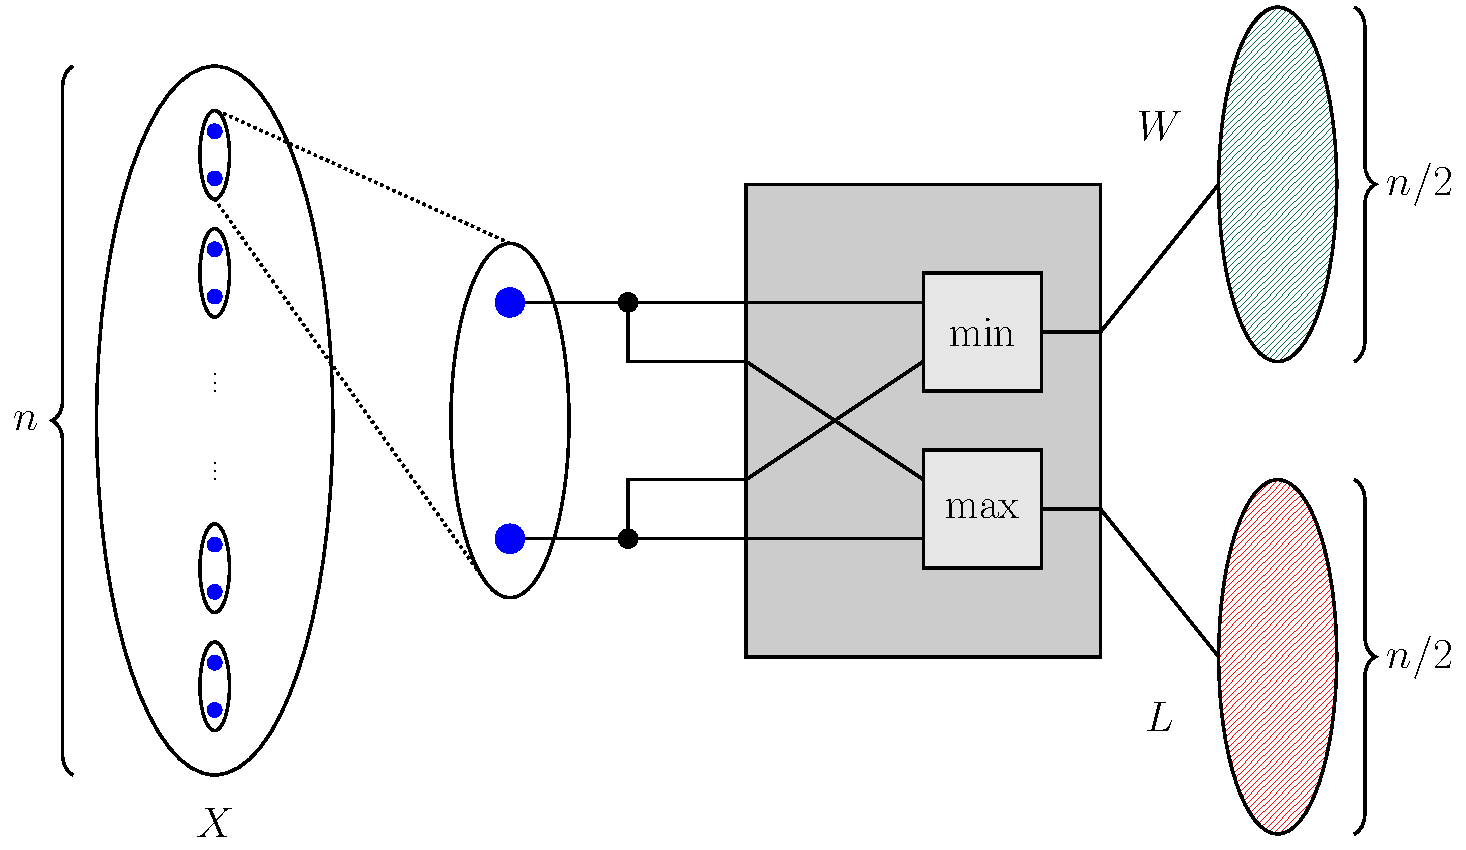
\includegraphics[scale=0.35]{snippets/tikz/min_p1.pdf}
        \vspace*{-4mm}
        \captionof{figure}{Visualisierung Phase 1}\label{fig: min_p1}
        %
        \vspace*{0.1cm}
\end{minipage}

\noindent\makebox[\linewidth]{\color{gray}{\hdashrule[0.5ex]{\linewidth}{0.5pt}{1.5mm}}}\\[.05cm]
% ---------------------------------------------------------------
%	Phase 2
\noindent
\begin{minipage}[Ht]{.34\textwidth}
\textbf{Phase 2.} In der zweiten Phase gilt aufgrund des ausbalancierten Turnierbaums $1 \leq f_{x_l}(n)\leq \log_2(k)$ $\forall x_l\in L$ und $f_{x_w}(n)=0$ $\forall x_w\in W$ sowie Insbesondere $\mfgm = 0$ und $\mfgr = \log_2(k)$.\\[.15cm]
\end{minipage}% This must go next to `\end{minipage}`
%
\hfill
%
\begin{minipage}[Ht]{.64\textwidth}
        \centering
        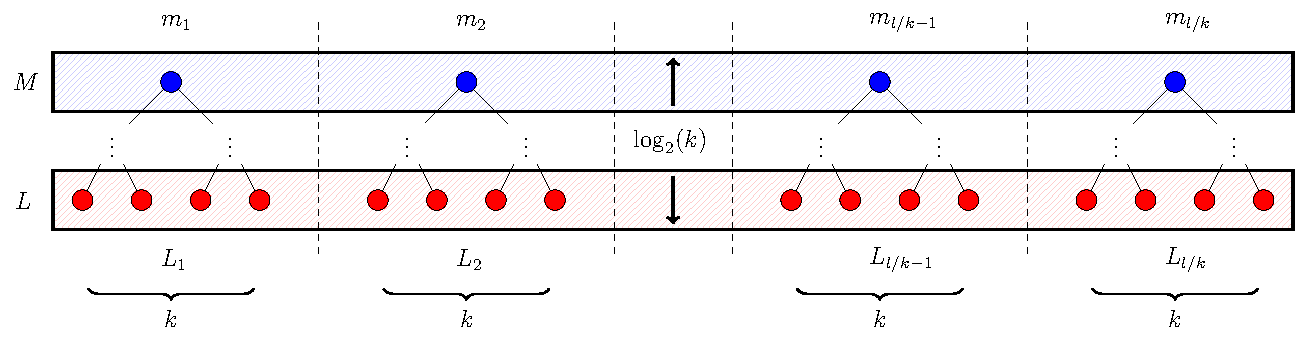
\includegraphics[scale=0.5]{snippets/tikz/min_p2.pdf}
        \vspace*{-10mm}
        \captionof{figure}{Visualisierung Phase 2}\label{fig: min_p1}
\end{minipage}
%
\noindent
Um in einem perfekt ausbalancierten Turnierbaum bei $k$ Teilnehmern einen Sieger zu ermitteln, bedarf es $k-1$ Vergleiche. Da es $n/2k$ Teilmengen gibt, ergibt sich $w(n)\leq (k-1)\cdot (n/2k) = n/2 - n/2k = \mO(n)$.\\[.05cm]
\noindent\makebox[\linewidth]{\color{gray}{\hdashrule[0.5ex]{\linewidth}{0.5pt}{1.5mm}}}\\[.05cm]
% ---------------------------------------------------------------
%	Phase 3
\noindent
\textbf{Phase 3.} In der dritten Phase wird jedes Element aus $W$ genau ein mal mit einem Element $m_i$ verglichen. Es gilt somit $f_{x_w}(n)=1$ $\forall x_w\in W$ sowie $f_{m_i}(n)\leq k$ $\forall m_i$.\\
Für die in Phase 3 verrichtete Arbeit gilt $w(n)\leq n/2 + k\cdot n/2=\mO(n)$.\\[.05cm]
\noindent\makebox[\linewidth]{\color{gray}{\hdashrule[0.5ex]{\linewidth}{0.5pt}{1.5mm}}}\\[.05cm]
% ---------------------------------------------------------------
%	Phase 4
\noindent
\textbf{Phase 4.} Die vierte Phase unterscheidet zwei Fälle. Wird die angegebene Schranke eingehalten, so gilt $1\leq f_{x_{w'}}(n)\leq \log_2(|W'|)$ $\forall x_{w'}\in W'$ sowie $f_e(n)=0$ $\forall e\notin W'$.\\
Insbesondere gilt $\mfgm = \log_2(|W'|)$ sowie $\mfgr = \log_2(|W'|)-1$.\\[.075cm]
In diesem Fall gilt für die verrichtete Arbeit $w(n)=|W'|-1=\mO(n)$.\\[.075cm]
Im zweiten Fall findet ein rekursiver Aufruf statt, sodass keinerlei Vergleiche stattfinden.
\\[.05cm]
\noindent\makebox[\linewidth]{\color{gray}{\hdashrule[0.5ex]{\linewidth}{0.5pt}{1.5mm}}}\\[.05cm]
% ---------------------------------------------------------------
%	Algo
\noindent
\textbf{RMinimum.} Für den gesamten Algorithmus ist relevant festzustellen, dass die Wahrscheinlichkeit, die Schranke der vierten Phase einzuhalten, von der Randomisierung der vorherigen Phasen abhängig ist. Dementsprechend ist die Mächtigkeit der Menge $|W'|$ bei wiederholter Ausführung mit gleicher Parametrisierung immer noch zufällig, wobei die stochastische Verteilung abhängig von der Wahl der Parameter ist.\\[.2cm]
Folgende Aussagen wollen wir im Laufe dieser Arbeit experimentell unterstützen.\\[.05cm]
\noindent\makebox[\linewidth]{\color{gray}{\hdashrule[0.5ex]{\linewidth}{0.5pt}{1.5mm}}}
% ---------------------------------------------------------------
%	Theoreme
%================================================================
\begin{manualtheorem}{3}\label{theo: min_3}
\Rm benötigt lineare Arbeit, also $w(n)=\mO(n)$.
\end{manualtheorem}
\begin{proof}
Betrachte einen beliebigen Rekursionsschritt mit einer Eingabemenge der Mächtigkeit $n'$. Die erste Phase benötigt $\mO(n')$ viele Vergleiche um die Mengen $W$ und $L$ zu bestimmen. Des Weiteren beinhaltet die Menge $W'$ kein Element der Menge $L$ und es folgt $w(n)= w(|W'|) + \mO(n) \leq w(n/2) + \mO(n) = \mO(n)$. 
\end{proof}
%================================================================
\begin{manuallemma}{2}\label{lem: min_2}
Sei $W_i$ eine beliebige Siegerpartition sowie $m_i$ das zum Filtern genutzte Minimum und $W'_i=\{w|w\in W_i \wedge w_i < m_i\}$ die Menge aller Elemente, die kleiner als $m_i$ sind.\\
Dann gilt $\mathbb{E}[|W'_i|]\leq 2d\sqrt{k}$ für eine Konstante $d>0$.
\end{manuallemma}
%================================================================
\begin{manualtheorem}{4}\label{theo: min_4}
Sei $k(n)=n^{\varepsilon}$ für $0<\varepsilon<1/2$. Dann benötigt \Rm $\mathbb{E}[f_{min}]=\mathcal{O}(\varepsilon^{-1}\log\log(n))$ Vergleiche für das \mE und $\mathbb{E}[f_{rem}]=\mathbb{O}(n^{\varepsilon})$ für alle übrigen Elemente.
\end{manualtheorem}
%================================================================
\begin{manualtheorem}{5}\label{theo: min_5}
Sei $k(n)=\log(n)/\log\log(n)$. Dann benötigt \Rm $\mathbb{E}[f_{min}]=\mathcal{O}(\log(n)/\log\log(n))$ Vergleiche für das \mE und $\mathbb{E}[f_{rem}]=\mathcal{O}(\log(n)/\log\log(n))$ für alle übrigen Elemente.
\end{manualtheorem}

\noindent\makebox[\linewidth]{\color{gray}{\hdashrule[0.5ex]{\linewidth}{0.5pt}{1.5mm}}}\\[.05cm]
% ---------------------------------------------------------------
%	Ende
\noindent
Die aufgeführten Theoreme und Lemmata dienen als Grundlage für den Analyseschwerpunkt und somit auch für die in dieser Arbeit zugrunde liegende Implementierung. 











		%	Analyse

\newpage

%================================================================
\label{4 : RMedian}				%	4 : RMedian
%----------------------------------------------------------------
%%%%%%%%%%%%%%%%%%%%%%%%%%%%%%%%%%%%%%%%%%%%%%%%%%%%%%%%%%%%%%%%%
\section{\RM}	%	RMEDIAN
%%%%%%%%%%%%%%%%%%%%%%%%%%%%%%%%%%%%%%%%%%%%%%%%%%%%%%%%%%%%%%%%%

Der Algorithmus \RM ist ein in Erwartung Praxis-optimaler Algorithmus zum Auffinden des Median Elements. Hierbei wird explizit auf die im Paper~\cite{meyer2} vorgestellte Version Bezug genommen.\\[.1cm]
Mit Hilfe eines Parameters $k(n)$ kann man den \trade zwischen der erwarteten \fg \fgM des Median Elements und der maximal erwarteten \fg \fgr aller übrigen Elemente kontrollieren. Dies erlaubt je nach Adjustierung des Parameters verschiedene Werte für das Paar \fgpair zwischen\\
$\langle\mathcal{O}(\log\log(n)),\mathcal{O}(\sqrt{n})\rangle$ und $\langle\mathcal{O}(\log(n)/\log\log(n)),\mathcal{O}(\log(n))\rangle$.

%%%%%%%%%%%%%%%%%%%%%%%%%%%%%%%%%%%%%%%%%%%%%%%%%%%%%%%%%%%%%%%%%			%	Einleitung
%%%%%%%%%%%%%%%%%%%%%%%%%%%%%%%%%%%%%%%%%%%%%%%%%%%%%%%%%%%%%%%%%
\subsection{Algorithmus}	%	RMEDIAN - Algorithmus
%%%%%%%%%%%%%%%%%%%%%%%%%%%%%%%%%%%%%%%%%%%%%%%%%%%%%%%%%%%%%%%%%
\RM erhält als Eingabe eine Menge $X$ mit $|X|=n$, $n\in\mathbb{N}$ sowie zwei weitere Parameter $k(n),d(n)\in\mR$ und liefert als Resultat den Median der Menge $X$.\\[.2cm]
Der Algorithmus kann in drei getrennte Phasen unterteilt werden.\\
Er beginnt mit der \textit{Sampling Phase}, die aus der Ursprungsmenge $X$ eine zufällige Teilmenge $S$ nimmt, diese sortiert und anschließend in Segmente unterteilt, deren Größe durch die Parameter $k(n)$ und $d(n)$ bestimmt wird. Da $S$ eine zufällige Teilmenge der Menge $X$ ist, besitzt die Menge $S$ in Erwartung den gleichen Median wie $X$. Dabei entstehen im Verlauf des Prozesses drei Teilmengen $L$, $C$ und $R$. Am Ende enthält die Menge $L$ Elemente kleiner, $R$ Elemente größer als der Median der Menge $S$ und $C$ gerade die Elemente, die im Bereich des Medians der Menge $S$ liegen und somit als Median-Kandidaten dienen.\\[.2cm]

%================================================================
%	Algorithmus
%%%%%%%%%%%%%%%%%%%%%%%%%%%%%%%%%%%%%%%%%%%%%%%%%%%%%%%%%%%%%%%%%
\label{algo: rmed_1}	%	ALGO - RMedian - Probing Phase
%%%%%%%%%%%%%%%%%%%%%%%%%%%%%%%%%%%%%%%%%%%%%%%%%%%%%%%%%%%%%%%%%

\begin{algorithm}[H]
	\SetAlgoLined
	\caption{\RM : Sampling phase}
	\textbf{procedure} \textsc{Sampling Phase}$(X=\{x_1,\cdots,x_n\},k(n),d(n))$\\
		\hspace*{.5cm} Randomly sample $k$ elements from $X$ and sort $S$ with AKS\\
		\hspace*{.5cm} Distribute $S$ into buckets $L_b,L_{b-1},\cdots,L_1,C,R_1,\cdots,R_{b-1},R_b$ as follows:\\
			\hspace*{1cm} set $n_0=2\sqrt{k\log(n)},n_1=3\sqrt{k\log(n)},n_i=d\cdot n_{i-1}$\\
			\hspace*{1cm} $C=S[k/2-n_0:k/2+n_0]$ median candidates\\
			\hspace*{1cm} $L_i=S[k/2-n_i:k/2-n_{i-1}]$ buckets of elements presumed smaller than median\\
			\hspace*{1cm} $R_i=S[k/2+n_{i-1}:k/2+n_i]$ buckets of elements presmued larger than median\\
	\textbf{return} $L,C,R$
\end{algorithm}

%%%%%%%%%%%%%%%%%%%%%%%%%%%%%%%%%%%%%%%%%%%%%%%%%%%%%%%%%%%%%%%%%
%
\vspace*{.4cm}
%
\noindent
Anschließend folgt die \textit{Probing Phase}, welche für die Filterung dieses Algorithmus verantwortlich ist. Hierbei wird die Menge $S$ aus der \textit{Sampling Phase} genutzt, um alle übrigen Elemente so zu Filtern, dass am Ende die Menge $C$ eine Teilmenge der Ursprungsmenge $X$ darstellt, mit Elementen in einer gewissen Intervall um den Median herum. Insbesondere beinhaltet diese Menge den Median selbst.\\[.2cm]
%%%%%%%%%%%%%%%%%%%%%%%%%%%%%%%%%%%%%%%%%%%%%%%%%%%%%%%%%%%%%%%%%
\label{algo: rmed_2}%	ALGO - RMedian - Sampling Phase
%%%%%%%%%%%%%%%%%%%%%%%%%%%%%%%%%%%%%%%%%%%%%%%%%%%%%%%%%%%%%%%%%

\begin{algorithm}[H]
	\SetAlgoLined
	\caption{\RM : Probing Phase}
	\textbf{procedure} \textsc{Probing Phase}$(L, C, R)$\\
	\For{$x_i\in X\backslash S$ in random order}{
		\For{$j\in[b-1,\cdots,1]$ in order}{
			$x_A\leftarrow$ arbitrary element in $L_j$ with fewest compares\\
			$c\leftarrow1$ if $x_A$ is marked else $2$\\
			\If{$x_i<x_A$}{
				add $x_i$ as new pivot to $L_{b+c}$ if $j<b-c$ and mark it, otherwise discard $x_i$\\
				stop processing $x_i$
			}
			$x_B\leftarrow$ arbitrary element in $R_j$ with fewest compares\\
			$c\leftarrow 1$ if $x_B$ is marked else $2$\\
			\If{$x_i>x_B$}{
				add $x_i$ as new pivot to $R_{b+c}$ if $j<b-c$ and mark it, otherwise discard $x_i$\\
				stop processing $x_i$
			}
		\tcp*{By now it is established that $S[k/2-n_1]\leq x_i \leq S[k/2+n_1]$}
		add $x_i$ as median candidate to $C$
		}
	}
	\textbf{return} $L,C,R$
\end{algorithm}
%
\vspace*{.4cm}
%
\noindent
Am Ende folgt die \textit{Cleaning Phase}, die den Abschluss des Algorithmus bildet. Bei unglücklicher Wahl der Sample-Menge $S$ muss der Algorithmus abgebrochen werden. Dies geschieht, wenn das Sample nicht repräsentativ für die gesamte Menge steht, der relative Median des Samples sich also stark von dem Realen unterscheidet. Dieser Fall tritt jedoch nur mit einer äußerst geringen Wahrscheinlichkeit auf. Entsprechend der Mächtigkeit der entstandenen Menge $C$ ruft der Algorithmus sich nun auf dieser Menge erneut auf, oder sortiert diese Menge mit dem \textit{AKS}-Algorithmus und gibt den Median aus.\\[.2cm]
%%%%%%%%%%%%%%%%%%%%%%%%%%%%%%%%%%%%%%%%%%%%%%%%%%%%%%%%%%%%%%%%%
\label{algo: rmed_3}%	ALGO - RMedian - Cleaning Phase
%%%%%%%%%%%%%%%%%%%%%%%%%%%%%%%%%%%%%%%%%%%%%%%%%%%%%%%%%%%%%%%%%

\begin{algorithm}[H]
	\SetAlgoLined
	\caption{\RM : Cleaning Phase}
	\textbf{procedure} \textsc{Cleaning Phase}$(L, C, R, n0)$\\
	\If{$\max(\sum_i|L_i|,\sum_i|R_i|)>n/2$}{
		\textbf{return} \textsc{DetMedian}$(X)$
		\tcp*{Partitioning too imbalanced $\Rightarrow$ median not in $C$}
	}

	$k=\sum_i(|L_i|-|R_i|)$\\
	\If{$k<0$}{
		add $k$ arbitrary elements from $\bigcup_i R_i$ to $C$
	}
	\Else{
		add $k$ arbitrary elements from $\bigcup_i L_i$ to $C$
	}
	\If{$|C|<\log^4(n0)$}{
		sort $C$ with AKS and \textbf{return} median
	}
	\textbf{return} \textsc{RMedian}$(C,k(n),b(n))$
\end{algorithm}
%
\vspace*{.4cm}
%

%%%%%%%%%%%%%%%%%%%%%%%%%%%%%%%%%%%%%%%%%%%%%%%%%%%%%%%%%%%%%%%%%
%================================================================
%	Ende
\noindent
Die Ausgabe des Algorithmus ist der Median der Eingabemenge $X$.
\newpage
%%%%%%%%%%%%%%%%%%%%%%%%%%%%%%%%%%%%%%%%%%%%%%%%%%%%%%%%%%%%%%%%%			%	Algorithmus
%%%%%%%%%%%%%%%%%%%%%%%%%%%%%%%%%%%%%%%%%%%%%%%%%%%%%%%%%%%%%%%%%
\subsection{Analyse}	%	RMEDIAN - Analyse
%%%%%%%%%%%%%%%%%%%%%%%%%%%%%%%%%%%%%%%%%%%%%%%%%%%%%%%%%%%%%%%%%


\noindent
Im diesem Abschnitt wird der Algorithmus \Rm im Gesamten und seine einzelnen Phasen theoretisch analysiert.\\
Hierbei ist die Auswahl der diskutierten Bereiche und Theoreme auf die für diese Arbeit relevanten Aussagen eingeschränkt. Für weitere Informationen sei hier auf das Paper~\cite{meyer2} verwiesen.\\[.1cm]
\noindent\makebox[\linewidth]{\color{gray}{\hdashrule[0.5ex]{\linewidth}{0.5pt}{1.5mm}}}\\[.05cm]
% ---------------------------------------------------------------
%	Phase 1
\noindent
\textbf{Phase 1.} In der ersten Phase des Algorithmus wird eine zufällige Teilmenge $S\subset X$ gebildet und mit dem \textit{AKS}-Algorithmus~\cite{aks} sortiert. Somit muss unterschieden werden, ob sich das Median Element zufällig in $S$ befindet oder nicht. Dies geschieht offensichtlich mit der Wahrscheinlichkeit $\mathbb{P}[med \in S]=|S| / |X| = k/n$.\\[.05cm]
In diesem Fall benötigt der Algorithmus durch \textit{AKS} $\mO(k\log_2(k))$ Vergleiche, wovon neben weiteren nicht-Median Elementen nun auch das Median Element selbst betroffen ist.\\
Andernfalls gilt dies nur für nicht-Median Elemente und insbesondere $f_{med}(n)=0$.\\[.1cm]
\noindent\makebox[\linewidth]{\color{gray}{\hdashrule[0.5ex]{\linewidth}{0.5pt}{1.5mm}}}\\[.05cm]
\textbf{Phase 2.} Die zweite Phase des Algorithmus filtert Elemente aus $X$, die als Median-Kandidat ausgeschlossen werden können. Des Weiteren ist festzustellen, dass sich das Median Element selbst am Ende der zweiten Phase definitiv in der Menge $C$ aller Median-Kandidaten befindet.\\
Es ist zu bemerken, dass für das Median Element selbst eine Fallunterscheidung zutrifft. Hat sich das Median Element in der in Phase 1 ausgewählten Teilmenge $S$ befunden, so befindet es sich, bis auf sehr wenige in Phase 3 abgefangene Ausnahmen, bereits in der Menge $C$. Somit wird es im Laufe der zweiten Phase nicht weiter verglichen und es gilt $f_{med}(n)=0$. Befand sich der Median jedoch nach der ersten Phase nicht in der Menge $S$, so wird er mit je einem Element aus jedem Behälter $L_i$ und $R_i$ in $L$ oder $R$ verglichen, sodass gilt $f_{med}(n)=|L| + |R| = b + b = 2\cdot b$.\\[.05cm]
Über die \fg aller übrigen Elemente lässt sich aufgrund der zufälligen Auswahl der Filter-Elemente keine Abschätzungen bilden.\\[.1cm]
\noindent\makebox[\linewidth]{\color{gray}{\hdashrule[0.5ex]{\linewidth}{0.5pt}{1.5mm}}}\\[.05cm]
\textbf{Phase 3.} Die dritte Phase des Algorithmus überprüft die Filterung der zweiten Phase und entscheidet anschließend, wie weiter verfahren wird. Wie in der ersten Phase findet auch hier kein Vergleich zwischen zwei Elementen statt. Anhand dessen wird entschieden, ob abgebrochen und der Median deterministisch bestimmt, die Menge mit dem \textit{AKS}-Algorithmus sortiert oder ein rekursiver Aufruf gestartet werden muss.\\[.1cm]
\noindent\makebox[\linewidth]{\color{gray}{\hdashrule[0.5ex]{\linewidth}{0.5pt}{1.5mm}}}\\[.05cm]
\textbf{RMedian.} Für den gesamten Algorithmus ist anzumerken, dass die Analyse für eine Eingabemenge $X$ der Größe $n\leq 2^{16}$ uninteressant ist. Dies liegt an der in Phase drei gegebenen Schranke für eine Sortierung mit dem \textit{AKS}-Algorithmus, denn für die entsprechende Ungleichung gilt $c \leq \log_2(n)^4$ $\forall c\leq n\leq 2^{16}$.\\[.1cm]
\noindent\makebox[\linewidth]{\color{gray}{\hdashrule[0.5ex]{\linewidth}{0.5pt}{1.5mm}}}

\begin{manuallemma}{26}\label{lem: med_26}
Die erwartete \fg des Medians \fgM ist

\[
\mathbb{E}[f_{med}(n)]=\mathbb{E}\left[f_{med}(\mO(\sqrt{n\log(n)}))\right]+\mO(\underbrace{\frac{k}{n}}_{\text{Sampled}}+\underbrace{(1-\frac{k}{n})\log_d(k)}_{\text{Not sampled}}+\underbrace{1}_{\text{Misclassified}}).
\]


\end{manuallemma}

\begin{manuallemma}{27}\label{lem: med_27}
Die erwartete \fg aller nicht-Median Elemente \fgr ist

\begin{center}
\begin{tabular}{lcl}
$\mathbb{E}[f_{rem}(n)]$&$=$&$\mathbb{E}\left[f_{rem}(\mO(\sqrt{n\log(n)}))\right]$\\
&$+$&$\mO(\underbrace{\log(k)}_{\text{Sampled}}+\underbrace{\log_d(n)}_{\text{Not sampled}}+\max(\underbrace{d^2}_{\substack{\text{Pivot in }R_i \\ i>2}}, \underbrace{\frac{nd}{k}}_{\substack{\text{Pivot in } R_j\\ j\leq 2}})),$
\end{tabular}
\end{center}
wobei $d(n)=\Omega(\log^{\varepsilon}(n))$ für ein $\varepsilon >0$ und $k(n)=\mO(n/\log(n))$.
\end{manuallemma}


\begin{manualtheorem}{28}\label{theo: med_28}
\RM erreicht $\mathbb{E}[f_{med}(n)] = \mO(\log\log(n))$ und $\mathbb{E}[f_{rem}(n)]=\mO(\sqrt{n})$.
\end{manualtheorem}
\begin{proof}
Wähle $k(n)=n^{\varepsilon}$, $d(n)=n^{\delta}$ mit $\varepsilon=2/3$, $\delta=1/12$. Nach Lemmata~\ref{lem: med_26} und ~\ref{lem: med_27} folgt:

\begin{center}
\begin{tabular}{lcl}
$\mathbb{E}[f_{med}(n)]$& $=$&$\mathbb{E}\left[f_{med}(\mO(\sqrt{n \log(n)}))\right]+\mO(n^{\varepsilon - 1} \varepsilon \log(n) + \frac{\varepsilon}{\delta}=\mO(\log\log(n))$,\\
$\mathbb{E}[f_{rem}(n)]$& $=$&$\mathbb{E}\left[f_{rem}(\mO(\sqrt{n \log(n)}))\right]+\mO((\varepsilon + \frac{1}{\delta})\log(n) + \max(2\delta, 1-\varepsilon + 2\delta))=\mO(\sqrt{n})$
\end{tabular}
\end{center}
\end{proof}



\begin{manualtheorem}{29}\label{theo: med_29}
\RM erreicht $\mathbb{E}[f_{med}(n)] = \mO(\frac{\log(n)}{\log\log(n)})$ und $\mathbb{E}[f_{rem}(n)]=\mO(\log(n))$.
\end{manualtheorem}
\begin{proof}
Wähle $k(n)=\frac{n}{\log^{\varepsilon}(n)}$, $d(n)=\log^{\delta}(n)$ mit $\varepsilon=\delta=1/3$. Nach Lemmata~\ref{lem: med_26} und ~\ref{lem: med_27} folgt:
\begin{center}
\begin{tabular}{lclcl}
$\mathbb{E}[f_{med}(n)]$& $=$&$\mathbb{E}\left[f_{med}(\mO(\sqrt{n \log(n)}))\right]$& $+$&$\mO(\log^{1-\varepsilon}(n) + \log_{\log^4(n)}(n))=\mO(\frac{\log(n)}{\log\log(n)})$,\\
$\mathbb{E}[f_{rem}(n)]$& $=$&$\mathbb{E}\left[f_{rem}(\mO(\sqrt{n \log(n)}))\right]$& $+$&$\mO(\log(n) + \max(\log^{2\delta}(n) + \log^{\varepsilon + \delta}(n))=\mO(\log(n))$
\end{tabular}
\end{center}

\end{proof}



\begin{manualtheorem}{30}\label{theo: med_30}
Für $k=\mO(n/\log(n))$ und $d=\Omega(\log(n))$, \RM benötigt in Erwartung insgesamt $\mO(n)$ Vergleiche. Dies impliziert eine erwartete Arbeit $w(n)=\mO(n)$.
\end{manualtheorem}

\noindent\makebox[\linewidth]{\color{gray}{\hdashrule[0.5ex]{\linewidth}{0.5pt}{1.5mm}}}\\[.05cm]
% ---------------------------------------------------------------
%	Ende
\noindent
Die aufgeführten Theoreme und Lemmata dienen als Grundlage für den Analyseschwerpunkt und somit auch für die zugrunde liegende Implementierung. 


		%	Analyse

\newpage
%%%%%%%%%%%%%%%%%%%%%%%%%%%%%%%%%%%%%%%%%%%%%%%%%%%%%%%%%%%%%%%%%
\section{Implementierung}	%	RMINIMUM - Implementierung
%%%%%%%%%%%%%%%%%%%%%%%%%%%%%%%%%%%%%%%%%%%%%%%%%%%%%%%%%%%%%%%%%

\noindent
In diesem Abschnitt wird die beiliegende Implementierung der Algorithmen \Rm und \RM vorgestellt und die Auswahl der Unittests sowie die Funktionalität weiterer beiliegender Dateien diskutiert.\\[.1cm]
Als grundlegende Programmiersprache wurde für beide Projekte \textit{Python} gewählt. Bei der Implementierung wurde weitestgehend auf externe Bibliotheken verzichtet, lediglich \textit{matplotlib} und \textit{pandas} zur Datenanalyse sowie \textit{PyTest} für beiliegende Testfälle wurden eingebunden.\\[.05cm]
Der vollständige Code dieser Arbeit ist bei \textit{Github}~\footnote{Github Repository: \href{https://github.com/jfklorenz/Bachelor-Thesis}{https://github.com/jfklorenz/Bachelor-Thesis}} veröffentlicht.  Für das gesamte Projekt sowie die einzelnen Algorithmen liegen \textit{README.md} Dateien zur besseren Strukturierung bei. An kritischen Stellen ist der gesamte Code einheitlich mit Kommentaren versehen, so dass hiermit auf die Ausführung einzelner Codesegmente verzichtet wird. 

%%%%%%%%%%%%%%%%%%%%%%%%%%%%%%%%%%%%%%%%%%%%%%%%%%%%%%%%%%%%%%%%%
%	Datenstruktur / Basics
\subsection{\Rm}
Sowohl der Algorithmus \Rm selbst als auch alle vier Phasen des Algorithmus liegen als separate Dateien vor und sind unabhängig voneinander ausführbar. Der Hauptanteil der Arbeit des Algorithmus besteht aus dem Bilden von Teilmengen einer gegebenen Menge sowie dem Bestimmen des Minimums einer Menge durch einen perfekt ausbalancierten Turnierbaum. Aus diesem Grund wurde zur Speicherung der Eingabemenge als Datentyp Listen gewählt. Diese erlauben ein unkompliziertes Aufteilen in Teilsegmente, wie bei \Rm in der zweiten und dritten Phase sowie bei \RM in der Ersten vonnöten. Des weiteren erlaubt der Index basierte Zugriff auf einzelne Elemente eine erleichterte Speicherung der Anzahl benötigter Vergleiche.\\[.05cm]
Die von \Rm  genutzten perfekt ausbalancierten Turnierbäume wurden mit Hilfe einer Warteschlange realisiert. Für einen Turnierbaum mit $n$ Elementen werden zunächst alle Elemente in einer Warteschlange gespeichert. Anschließend werden nach dem \textit{First-In-First-Out} Prinzip zwei Elemente entnommen und miteinander verglichen. Das kleinere der beiden Elemente wird daraufhin wieder in die Warteschlange eingefügt. Dieser Vorgang wird so lange wiederholt, bis sich nur noch ein einziges, als Turniersieger deklariertes Element in der Warteschlange befindet. Der Vorteil dieses Verfahren ist, dass nur eine Warteschlange der Länge $n$ und keine rekursiven Aufrufe benötigt werden.\\[.05cm]
Die Anzahl der Vergleiche, an denen jedes Element teilgenommen hat, wird für jedes Element separat gespeichert.

\subsection{\RM}
Für \RM liegt ebenfalls der Algorithmus wie auch die drei Phasen als separate Dateien vor. Da auch dieser Algorithmus mit dem Aufteilen von Mengen anhand von Indizes arbeitet, wurde auch hier als Datentyp Listen gewählt. Dies erlaubt zusätzlich eine hohe Konsistenz in der Auswertung beider Algorithmen und ihrer gespeicherten Daten.
Für jedes Element werden zum einen die Anzahl der Vergleiche gespeichert, an denen es teilgenommen hat, und zum anderen die in der zweiten Phase auftretende Markierung gespeichert.

\noindent
Der Code beider Algorithmen liegt der Arbeit in elektronischer Form bei, ist jedoch auszugsweise angehängt. Da der Schwerpunkt dieser Arbeit auf der Auswertung der Daten liegt und der Code an entsprechenden Stellen kommentiert wurde, wird hier auf weitere Ausführungen bezüglich der exakten Implementierung verzichtet.

%%%%%%%%%%%%%%%%%%%%%%%%%%%%%%%%%%%%%%%%%%%%%%%%%%%%%%%%%%%%%%%%%
%	Unittests
\subsection{Modultests}
Für die experimentelle Auswertung dieser Arbeit ist es notwendig zu garantieren, dass die Vorliegende Implementierung funktional arbeitet. Um dies zu gewährleisten wurden im Vorfeld Modultests durchgeführt.

% ===============================================================
\subsubsection{PyTest}
Für die reine Validierung einzelner Codesegmente und für die Korrekte Ausgabe des Minimums beziehungsweise Medians wurde \textit{PyTest} gewählt.\\[.05cm]
Neben der Möglichkeit einer freien Parametrisierung der Testfälle liegen bereits vordefinierte Eingaben bei. Diese beinhaltet zum einen eine randomisierte Parametrisierung und zum anderen ihrem Definitionsbereich nach extreme Belegungen.\\[.1cm]

\noindent
Für den Algorithmus \Rm wurde Für Phase 1 getestet, ob die Mengen $W$ und $L$ gleich mächtig und das Minimum in $W$ enthalten ist. Des weiteren wird garantiert, dass jedes Element an genau einem Vergleich teilgenommen hat.\\[.03cm]
Für Phase 2 wird zunächst die korrekte Größe der Teilmengen geprüft. Anschließend wird validiert, dass jedes Element an maximal $\lceil \log_2(k)\rceil$ Vergleichen teilgenommen hat sowie das Minimum an exakt so vielen.\\[.03cm]
Für Phase 3 ist gewährleistet, dass die Größe der Teilmengen und die eine sinngemäße Filterung eingehalten wird. Ebenso wird die vorgesehene Anzahl an Vergleichen stets exakt eingehalten.\\[.03cm]
Für Phase 4 muss lediglich das korrekte Einhalten der gegebenen Schranke überprüft werden.\\[.1cm]
Anschließend wurde der gesamte Algorithmus auf die korrekte Ausgabe des Minimums beziehungsweise Medians hin getestet. Insbesondere sei hier hervorzuheben, dass für die geleistete Arbeit $w(n)$ des Algorithmus \Rm auch für eine randomisierte Parametrisierung stets die Gleichung $n/2 \leq w(n) \leq 2\cdot n$ eingehalten wurde. Dies bestärkt Theorem~\ref{theo: min_3}.\\[.1cm]

\noindent
Die Gestaltung der Modultests für den Algorithmus \RM ist jedoch komplexer. Dies liegt primär an der Tatsache, dass es auf rein theoretischer Basis sehr aufwendig ist, eine gültige Eingabe für die zweite Phase zu generieren. Aus diesem Grund wurde zuerst Phase 1 des Algorithmus validiert. Anstatt nun anschließend die zweite Phase allein zu testen, wurden die ersten beiden Phasen nun zusammen durchlaufen.\\[.03cm]
Für Phase 1 wurde die korrekte Konstruktion der Mächtigkeit aller Teilmengen $L_i$, $R_i$, $L$, $C$ und $R$ getestet.\\[.03cm]
Für Phase 2 wurde überprüft, ob sich der Median am Ende tatsächlich in der Menge $C$ der Median-Kandidaten befindet. Außerdem wurde gewährleistet, dass die \fg des Medians \fgM nicht größer ist als die Anzahl der linken und rechten Behälter beziehungsweise Mengen, also $f_{med}(n) \leq |L| + |R| = 2\cdot b$.\\[.03cm]
Für Phase 3 wurden für jeden der drei möglichen Ausgänge Eingaben konzipiert, um zu kontrollieren, ob immer eine korrekte Auswahl getroffen wurde.

% ===============================================================
\subsubsection{Jupyter Notebook}
Um die korrekte Auswertung der \fg $f(n)$ und der Arbeit $w(n)$ zu gewährleisten, liegen ausführlichere Experimentalfälle als \textit{Jupyter Notebook} Dateien bei. Diese erlauben eine schnelle Reproduzierbarkeit einzelner Experimente.\\
Insbesondere liegen für die hier diskutierten Theoreme spezielle Dateien bei, die es dem Nutzer ermöglichen sollen, deren Aussagen für manuelle Eingaben effizient zu überprüfen.

%%%%%%%%%%%%%%%%%%%%%%%%%%%%%%%%%%%%%%%%%%%%%%%%%%%%%%%%%%%%%%%%%
\subsection{Werkzeuge}
Im Laufe dieser Arbeit sind ein paar zusätzliche Funktionalitäten implementiert worden, die den Umgang mit den Daten erleichtern sollen.\\[.05cm]
Da zur empirischen Auswertung oft nur bedingte Zeitintervalle zur Verfügung stehen bietet die beiliegende \textit{Python} Datei \textit{merge.py} die Option, in verschiedenen \textit{.csv}-Datei gespeicherte Daten der gleichen Eingabe in Form von \textit{Pandas DataFrames} zu einer einzigen, korrekt benannten Datei zusammenzufügen.\\[.1cm]
Des Weiteren liegen alle Methoden bei die benötigt werden, um die in dieser Arbeit verwendeten Grafiken zu reproduzieren oder für andere Datensätze neu auswerten zu können.\\[.1cm]
Zuletzt werden in dieser Arbeit wiederholt Datensätze gegen eine bestimmte Funktion gefittet. Dies wurde durch beiliegende \textit{Gnuplot}-Dateien realisiert und kann für neue Datensätze flexibel angepasst werden.\\[.1cm]
Für weitere Informationen bezüglich eines beiliegenden Werkzeugs sei hier auf die entsprechende \textit{README.md} verwiesen. 





\newpage

%================================================================
\label{5 : Testfälle}			%	5 : Testfälle
%----------------------------------------------------------------
%%%%%%%%%%%%%%%%%%%%%%%%%%%%%%%%%%%%%%%%%%%%%%%%%%%%%%%%%%%%%%%%%
\section{Experimentalfälle}		%	TESTFÄLLE - Test
%%%%%%%%%%%%%%%%%%%%%%%%%%%%%%%%%%%%%%%%%%%%%%%%%%%%%%%%%%%%%%%%%

\noindent
Die primäre Aufgabe dieser Arbeit ist die experimentelle Auswertung der Algorithmen \Rm und \RM und die Analyse der Resultate. In diesem Abschnitt wird zunächst diskutiert, was der Fokus der Analyse für beide Algorithmen ist und wie entsprechend unsere Auswahl an Experimentalfällen ausfällt.  Hierbei werden wir uns gegebenenfalls auf die in den entsprechenden Kapiteln vorgestellten Theoreme und Lemmata berufen. Zuletzt werden die genutzten Analysewerkzeuge kurz vorgestellt.\\[.1cm]

%%%%%%%%%%%%%%%%%%%%%%%%%%%%%%%%%%%%%%%%%%%%%%%%%%%%%%%%%%%%%%%%%
\noindent
Für beide Algorithmen sind die \fg der Algorithmen $f(n)$, die des Minimums \fgm oder Medians \fgM und die aller nicht-Minimum beziehungsweise nicht-Median Elemente von Bedeutung und somit auch die gesamt verrichtete Arbeit $w(n)$ beider Algorithmen.\\\\[.05cm]
Hierbei wird sich auf die Aussagen für den Algorithmus \Rm von Lemma~\ref{lem: min_2} sowie die Theoreme~\ref{theo: min_3}, ~\ref{theo: min_4} und ~\ref{theo: min_5} bezogen und versucht, diese experimentell zu unterstützen.\\
Analoges gilt bezüglich des Algorithmus \RM für die Theoreme~\ref{theo: med_28}, ~\ref{theo: med_29} und ~\ref{theo: med_30}.\\[.05cm]
Für den Algorithmus \RM wird sich auf die experimentelle Unterstützung der Theoreme~\ref{theo: min_4} und ~\ref{theo: min_5} beschränkt.\\[.05cm]
Die ersten drei Phasen von \Rm sowie die ersten beiden Phasen von \RM entsprechen einer randomisierten Filterung der Eingabemenge. Das Verhältnis von der Mächtigkeit der Eingabemenge und von der Mächtigkeit der gefilterten Menge entspricht einer Zufallsvariablen $\Delta X\in[0,1]$. Inwiefern diese von den Eingabeparametern den entsprechenden Algorithmen abhängt sowie ihre Verteilung, ist abschließend Bestand der Analyse.\\[.1cm]

%%%%%%%%%%%%%%%%%%%%%%%%%%%%%%%%%%%%%%%%%%%%%%%%%%%%%%%%%%%%%%%%%
%	Technik
\noindent
Die bereits diskutierte Implementierung der jeweiligen Algorithmen wurde im Vorfeld auf dem Hochleistungsrechner \textit{Goethe-HLR} der Goethe Universität Frankfurt am Main ausgeführt. Dabei handelt es sich um einen Computer Cluster basierend auf einer Intel CPU Architektur mit einem \textit{Scientific Linux 7.6} Betriebssystem.\\
Für eine optimale Nutzung des Servers wäre eine Parallelisierung des Codes vorteilhaft gewesen. Dies ist durch die rekursiven Aufrufe innerhalb der Algorithmen jedoch nicht möglich. Aus diesem Grund wurde die wiederholte Ausführung einzelner experimenteller Fälle parallel ausgeführt. Die Ergebnisse wurden in der Arbeit beiliegenden \csv gespeichert und anschließend lokal ausgewertet.\\[.1cm]


%%%%%%%%%%%%%%%%%%%%%%%%%%%%%%%%%%%%%%%%%%%%%%%%%%%%%%%%%%%%%%%%%
%	Testfälle
\noindent
Beide Algorithmen besitzen als Eingabe die Parameter $X$ und $k(n)$, wobei $X$ eine Menge mit strikter Totalordnung und $k(n)$ einen ganzzahligen Parameter darstellt. Ebenso nutzen beide Algorithmen in der zweiten und dritten Phase die Verhältnismäßigkeiten zwischen $n$ und $k(n)$ zur Bestimmung der Teilmengengröße. Aus diesem Grund wurde sich bei den hier präsentierten Daten für eine einheitliche Struktur der Eingaben entschieden, um ihre Vergleichbarkeit untereinander gewährleisten zu können.\\[.05cm]
Für die Menge $X$ der Eingabe wurde o.B.d.A. für beide Algorithmen $X=\{0,\cdots,n-1\}$, $n=2^i$, $i,k(n)\in\mN$ gewählt. Die spezifische Wahl des Parameters $k(n)$ sowie des Parameters $d$ des Algorithmus \RM wird an entsprechender Stelle genauer ausgeführt.\\
Für den Algorithmus \Rm wurde jeder Fall zehntausend mal, für \RM unterschiedlich oft ausgeführt. Die in den folgenden Kapiteln angeführten Grafiken visualisieren stets alle Ausführungen einer festen Eingabe oder den Verlauf bei Änderung eines Parameters. In letzterem Fall wurde stets der Mittelwert aller Wiederholungen der entsprechenden Eingabe als Repräsentant für die Darstellung gewählt.\\[.1cm]

%%%%%%%%%%%%%%%%%%%%%%%%%%%%%%%%%%%%%%%%%%%%%%%%%%%%%%%%%%%%%%%%%
%	Methoden
\noindent
Nun gilt es, die experimentellen Daten mit den Prognosen der entsprechenden Theoreme und Lemmata abzugleichen. Um mit ausreichender Gewissheit eine Aussage annehmen oder ablehnen zu können, muss insbesondere eine aussagekräftige Unterscheidung zwischen einer einfach-logarithmischen und einer doppelt-logarithmischen Entwicklung getroffen werden.\\[.05cm]
Für die benötigte nicht-lineare Regression wurde das Programm \textit{Gnuplot}~\cite[S.74-81]{gnu} genutzt. Dieses nutzt den Marquardt-Levenberg~\cite[S.65-68]{gnu2} Algorithmus zur Ausgleichsrechnung, um mit Hilfe der Methode der kleinsten Quadrate einen passenden Fit zu bestimmen. Die Auswertung der Fits sowie die Wahl der Parameter liegen der Arbeit als \textit{.txt}-Datei bei.



%%%%%%%%%%%%%%%%%%%%%%%%%%%%%%%%%%%%%%%%%%%%%%%%%%%%%%%%%%%%%%%%%

%%%%%%%%%%%%%%%%%%%%%%%%%%%%%%%%%%%%%%%%%%%%%%%%%%%%%%%%%%%%%%%%%
\subsection{\Rm}		%	TESTFÄLLE - RMin
%%%%%%%%%%%%%%%%%%%%%%%%%%%%%%%%%%%%%%%%%%%%%%%%%%%%%%%%%%%%%%%%%
\noindent
Wir werden nun die experimentellen Auswertungen des Algorithmus \Rm besprechen. Interessant ist, hierbei festzustellen, wie genau die im Paper~\cite{meyer1} aufgeführten Schranken in der Praxis für den gesamten Algorithmus halten. Des Weiteren besteht ein besonderes Interesse an der Güte der Filterung der Phasen 1-3 innerhalb eines Rekursionsschrittes, da diese einen maßgeblichen Einfluss auf die Anzahl der insgesamt benötigten Rekursionsaufrufe aufweist.\\[.1cm]

%%%%%%%%%%%%%%%%%%%%%%%%%%%%%%%%%%%%%%%%%%%%%%%%%%%%%%%%%%%%%%%%%
			%	Einleitung
%%%%%%%%%%%%%%%%%%%%%%%%%%%%%%%%%%%%%%%%%%%%%%%%%%%%%%%%%%%%%%%%%
\subsubsection{Filter}		%	TESTFÄLLE - Filter
%%%%%%%%%%%%%%%%%%%%%%%%%%%%%%%%%%%%%%%%%%%%%%%%%%%%%%%%%%%%%%%%%

\noindent
Wir werden nun das Zusammenwirken der ersten drei Phasen von \Rm genauer untersuchen. Hierbei ist der Zusammenhang zwischen einzelnen Parametern und der Güte der Filterung besonders interessant.\\[.1cm]

%	Güte der Filter, ZV
\noindent
Wir definieren nun $\Delta X=|W'|/|X|=|W'|/n$ als die Güte der Filterung. Dies entspricht dem prozentualen Verhältnis zwischen der wie in Phase 3 festgelegten Mächtigkeit der Menge $W'$ und der Mächtigkeit $n$ der Eingabemenge $X$. Wir wissen, dass die Menge $W'$ zum einen das Minimum und zum anderen kein Element der Menge $L$ enthält. Es gilt $1 \leq |W'| \leq |X|/2=n/2$ und somit $0 < \Delta X \leq 1/2$. \\[.05cm]

\noindent
Bei einer Anzahl von $rep$ Wiederholungen besitzt $\Delta X$ die absolute Häufigkeit $H_{rep}(\Delta X)= \sum_{rep} \mathbbm{1}_{\Delta X}$. Die für uns interessanten Begrifflichkeiten der \textit{relativen Häufigkeit}, des \\
\textit{(Stichproben-) Mittelwertes} und der \textit{(Stichproben-) Varianz} ergeben sich nun über:
\begin{center}
\begin{tabular}{llcl}
\textbf{Relative Häufigkeit:}&$h_{rep}(\Delta X)$& $=$& $H_{rep}(\Delta X) / rep$\\[.25cm]
\textbf{Stichprobenmittelwert:}&$\Delta\overline{X}$& $=$ & $\frac{1}{rep}\sum_{rep} \Delta X$\\[.25cm]
\textbf{Stichprobenvarianz:}&$Var[\Delta X]$ & $=$ & $\sum\limits_{i=1}^{rep} (\Delta X_i - \overline{\Delta X})^2 \cdot h_{rep}(\Delta X)$
\end{tabular}
\end{center}

\noindent
Da der Wert von $\Delta X$ von der Randomisierung der Phasen 1-3 abhängig ist, kann er als Zufallsvariable mit Wertebereich $(0,1/2]$ aufgefasst werden.\\[.05cm]


%%%%%%%%%%%%%%%%%%%%%%%%%%%%%%%%%%%%%%%%%%%%%%%%%%%%%%%%%%%%%%%%%
\noindent
\begin{minipage}[Ht]{.45\textwidth}
Führt man den Algorithmus mit gleicher Eingabe wiederholt aus, so erwartet man nach dem (schwachen) Gesetz der großen Zahlen eine resultierende Normalverteilung der Ergebnisse. Wie in Abbildung~\ref{fig: min_GgZ} zu sehen ist mit steigender Anzahl an Wiederholungen immer klarer eine glockenförmige Darstellung der Verteilung der relativen Häufigkeiten $h_{rep}(n)$ zu erkennen. Hierbei sei anzumerken, dass bei einer solchen Darstellung der visuelle Trugschluss entsteht, dass sowohl der Extrempunkt als auch die Fläche unter der vermeintlichen Kurve zu sinken scheinen.\\[.1cm]
\end{minipage}% This must go next to `\end{minipage}`
%
\hfill
%
\begin{minipage}[Ht]{.54\textwidth}
        \centering
        \vspace*{-0.5cm}
        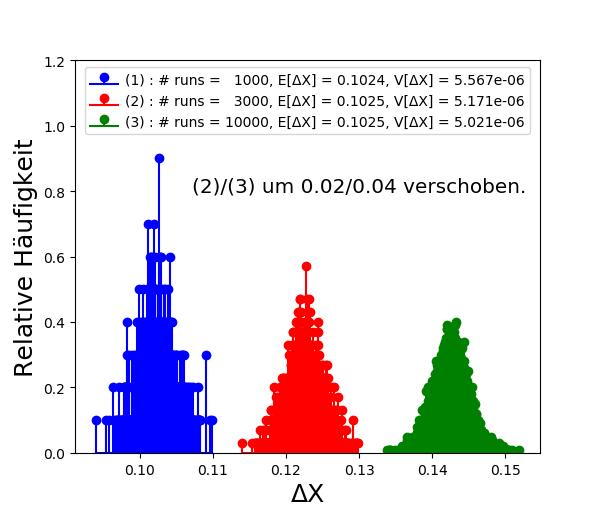
\includegraphics[scale=.66]{pictures/min_filter_runs.png}
   		\vspace*{-8mm}
   		\captionof{figure}{$\log_2(n) = 16$, $k = 64$}\label{fig: min_GgZ}

\end{minipage}

%%%%%%%%%%%%%%%%%%%%%%%%%%%%%%%%%%%%%%%%%%%%%%%%%%%%%%%%%%%%%%%%%
\noindent
Dies ist der diskreten Natur von Messwerten geschuldet. Bei einer Normalverteilung entspricht der Extrempunkt der Dichtefunktion dem Erwartungswert der zugehörigen Zufallsvariablen. Die in der Abbildung mit angegebenen Werte dienen zur Verdeutlichung der realen Entwicklung.\\[.05cm]
Von einer zugrunde liegenden Normalverteilung ausgehend wird versucht anhand der Parameter Abschätzungen für den Erwartungswert und die Varianz zu bilden.\\[.1cm]

\noindent
Um die Abhängigkeiten zu einzelnen Parametern getrennt nachzuweisen wurde für die Eingabe der Form $(n,k)$ stets einer der beiden Parameter fixiert, während für den anderen verschiedene Werte durchlaufen wurden. Dies erlaubt bestehende Korrelationen zu dem variablen Parameter zu erkennen. Für jeden hier erwähnten Fall wurden ohne anderweitige Angabe jeweils zehntausend Durchläufe ausgeführt und die Ergebnisse von $\Delta X$ separat gespeichert.\\[0.05cm]

\noindent
Im Folgenden wird die relative Häufigkeit mit $h(n)$, der Mittelwert mit $\mu$ sowie die Varianz mit $V(n,k)$ bezeichnet. Die relative Häufigkeit entspricht graphisch der Dichtefunktion der Zufallsvariable $\Delta X$.

%%%%%%%%%%%%%%%%%%%%%%%%%%%%%%%%%%%%%%%%%%%%%%%%%%%%%%%%%%%%%%%%%
%	Erwartungswert
% ---------------------------------------------------------------
%	ABHÄNGIGKEIT von N
\subsubsection*{Erwartungswert}
Nun soll die Abhängigkeit des Erwartungswertes von den Parametern $n$ und $k(n)$ untersucht werden. Hierzu wird zuerst der Parameter $k$ nacheinander auf verschiedene Werte fixiert und die Veränderung des Erwartungswertes abhängig von $n$ gemessen.\\[.1cm]
Den präsentierten Grafiken liegt die Fixierung von $k\in\{4, 32, 256\}$ für $\log_2(n)\in\{9,\cdots, 20\}$ zugrunde.

% ---------------------------------------------------------------
%	FIG: Abhängigkeit von N
\begin{figure}[H]
	%
    \hspace*{-1cm}
    \begin{minipage}[t]{.30\textwidth}
        \centering
        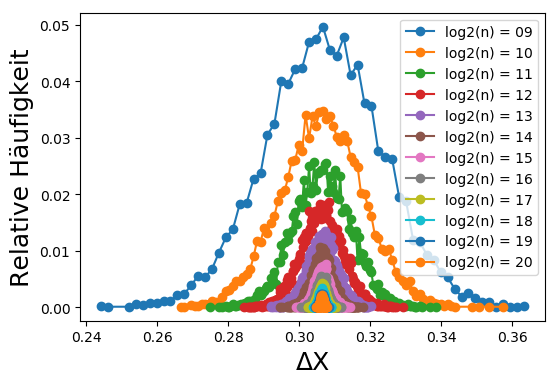
\includegraphics[width=1.2\textwidth]{pictures/min_filter_D_n_4.png}
    \end{minipage}
	%    
    \hspace*{0.8cm}
	%    
    \begin{minipage}[t]{.30\textwidth}
        \centering
        \raisebox{0.05cm}{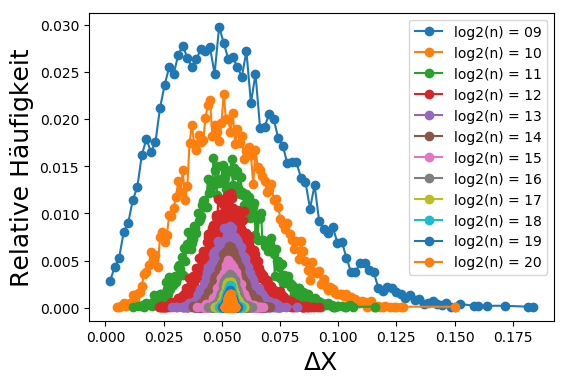
\includegraphics[width=1.21\textwidth]{pictures/min_filter_D_n_256.png}}
    \end{minipage}  
        \hspace*{0.8cm}
    \begin{minipage}[t]{.30\textwidth}
        \centering
        \raisebox{-0.05cm}{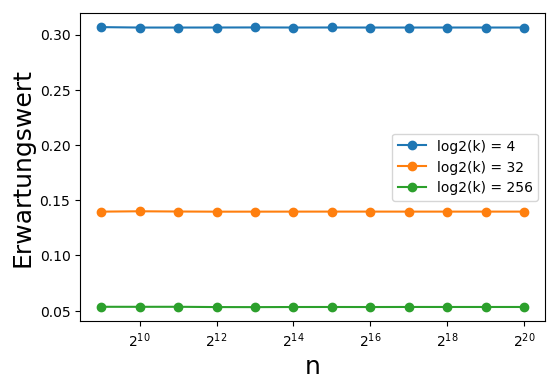
\includegraphics[width=1.2\textwidth]{pictures/min_filter_E_n}}
    \end{minipage}
    \captionof{figure}{$h(n)$ für $k=4$ und $k=256$ sowie $\mu$ für $k=4,32, 256$.}\label{fig: min_E_n}
\end{figure}

% ---------------------------------------------------------------
\noindent
Wie in Abbildung~\ref{fig: min_E_n} eindeutig zu erkennen, ist bleibt der Erwartungswert nach Fixierung von $k$ konstant für alle Werte für $n$.\\[.1cm]

% ===============================================================
%	ABHÄNGIGKEIT von K
\noindent
Nun wird der Parameter $n=2^{16}$ fixiert und alle Werte für $k=2^i$, $i\in\mN$, $k<n$ untersucht.\\

\noindent
Diesbezüglich wird sich nun auff die Aussage von Lemma~\ref{lem: min_2} berufen. Demnach gilt $\mathbb{E}[|W'_i|]\leq 2d\sqrt{k}$ für eine Konstante $d>0$. Insgesamt existieren $n/2k$ Teilmengen, womit folgt:
\[
\frac{|W'|}{|X|}=\frac{1}{n}\cdot \sum\limits_{i=1}^{n/k}\mathbb{E}[|W'_i|]=\frac{1}{n}\cdot \frac{n}{2k} \cdot \mathbb{E}[|W'|]\leq\frac{1}{2k}\cdot 2d\sqrt{k}=\frac{d}{\sqrt{k}}
\]

\noindent
Anhand der empirischen Daten wurde nun  mithilfe des Programms Gnuplot~\cite{gnu} versucht ein möglicher Fit für eine Abschätzung von $\mathbb{E}[\Delta X]$ zu berechnen.

% ---------------------------------------------------------------
%	FIG: Abhängigkeit von K
\begin{figure}[H]
    \hspace*{-0.8cm}
    \begin{minipage}[t]{.30\textwidth}
        \centering
        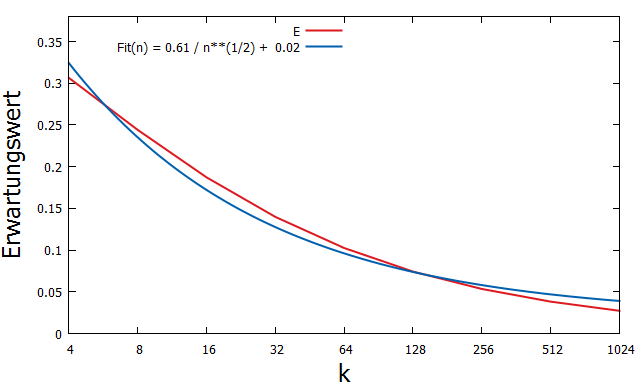
\includegraphics[width=1.2\textwidth]{pictures/min_filter_D_k.png}
    \end{minipage}
    \hspace*{.8cm}
    \begin{minipage}[t]{.30\textwidth}
        \centering
		\raisebox{-0.23cm}{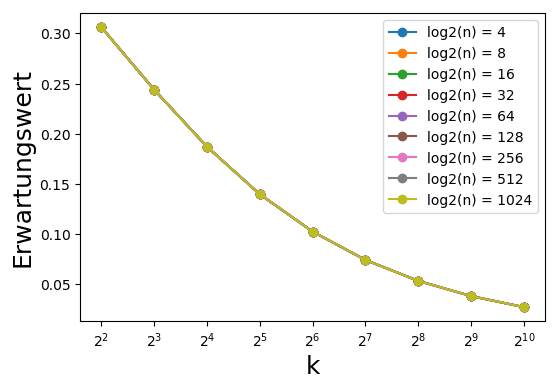
\includegraphics[width=1.1\textwidth]{pictures/min_filter_E_k.png}}
    \end{minipage}  
    \hspace*{.5cm}
    \begin{minipage}[t]{.30\textwidth}
        \centering
        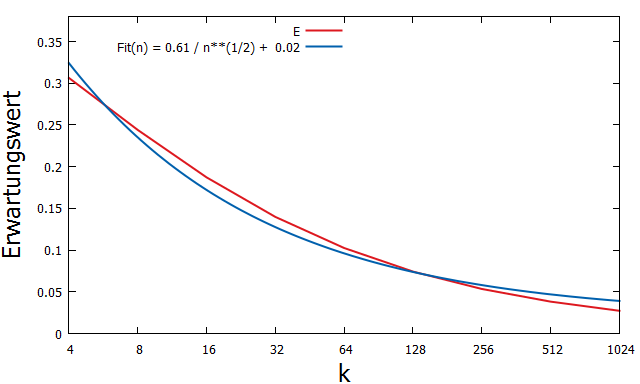
\includegraphics[width=1.2\textwidth]{pictures/min_filter_fit_E_k}
    \end{minipage}
    \captionof{figure}{$h(n)$ und $\mu$ für $\log_2(n)=16$, $\log_2(k)\in\{1,\cdots,15\}$ sowie Fit für $\mu$.}\label{fig: min_E_k}
\end{figure}

% ---------------------------------------------------------------
\noindent
Als Fit Funktion wurde hierfür $F_E(k)= a / \sqrt{k} + b$ und als Startwerte $a=0.5$ sowie $b=0.01$ gewählt. Nach 5 Iterationen ist der Fit konvergiert und die finale Summe der Residuenquadrate betrug $0.0011$. Es ergab sich eine Parametrisierung von $0.61$ und $b=0.03$. Vergleichbare Experimente ergaben ähnliche Ergebnisse, was die Aussage von Lemma~\ref{lem: min_2} bestätigt.\\[.1cm]
%%%%%%%%%%%%%%%%%%%%%%%%%%%%%%%%%%%%%%%%%%%%%%%%%%%%%%%%%%%%%%%%%
%	VARIANZ
% ---------------------------------------------------------------
%	ABHÄNGIGKEIT von N
\subsubsection*{Varianz}
Nun kann die Abhängigkeit der Varianz von den Parametern $n$ und $k(n)$ untersucht werden.\\[.1cm]
Wie schon beim Erwartungswert wird mit der Abhängigkeit von $n$ begonnen und $k$ dafür auf verschiedene Werte fixiert. Für eine direkte Vergleichbarkeit wurde für die Grafiken der gleiche Datensatz genutzt.

% ---------------------------------------------------------------
%	FIG: Abhängigkeit von N
\begin{figure}[H]
    \hspace*{-1cm}
    \begin{minipage}[t]{.30\textwidth}
        \centering
        \raisebox{-0.15cm}{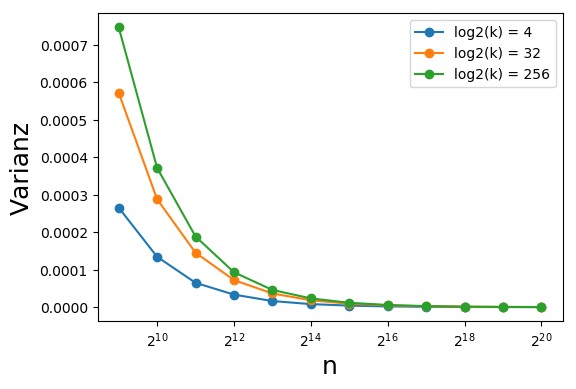
\includegraphics[width=1.1\textwidth]{pictures/min_filter_V_n.png}}
    \end{minipage}
    \hspace*{0.5cm}
    \begin{minipage}[t]{.30\textwidth}
        \centering
        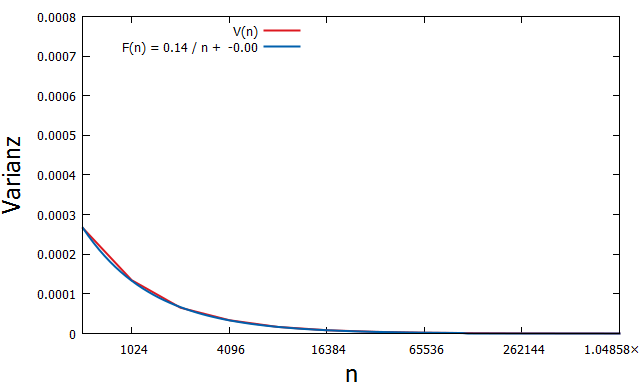
\includegraphics[width=1.2\textwidth]{pictures/min_filter_fit_V4_n.png}
    \end{minipage}  
    \hspace*{0.8cm}
    \begin{minipage}[t]{.30\textwidth}
        \centering
        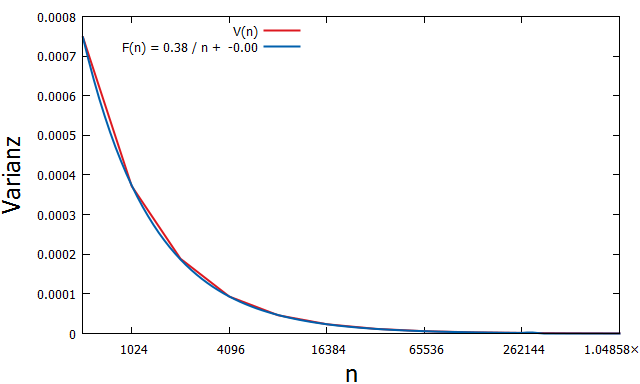
\includegraphics[width=1.21\textwidth]{pictures/min_filter_fit_V256_n.png}
        
    \end{minipage}
    \vspace*{-0.1cm}
    \captionof{figure}{$V(n)$ für $k\in\{4,32,256\}$ sowie Fit für $k\in\{4,256\}$.}\label{fig: min_V_n}
\end{figure}

% ---------------------------------------------------------------
\noindent
Wie in Abbildung~\ref{fig: min_V_n} zu sehen ähnelt der Verlauf der Varianz $V(n)$ dem einer Hyperbel. Der Fit wurde dementsprechend mit $F_V(n)=a/n + b$ mit den Startwerten $a=0.4$ und $b=0.0000001$ gewählt. Nach 5 Iterationen ist der Fit konvergiert. Die finale Summe der Residuenquadrate und weitere relevante Parameter liegen dieser Arbeit bei. Anzumerken ist hier, dass
sich die Parametrisierung von $b=0$ für alle experimentellen Werte von $k$ ergab.\\[.1cm]

\noindent
% ---------------------------------------------------------------
%	ABHÄNGIGKEIT von K
Abschließend wird noch die Abhängigkeit der Varianz $V(n,k)$ von dem Parameter $k$ geprüft und $n$ wie bereits zuvor auf $\log_2(n)=16$ fixiert.

% ---------------------------------------------------------------
%	FIG: Abhängigkeit von K
\begin{figure}[H]
    \hspace*{-1cm}
    \begin{minipage}[t]{.30\textwidth}
        \centering
        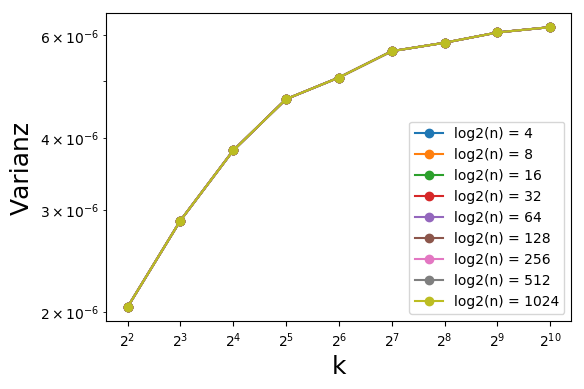
\includegraphics[width=1.2\textwidth]{pictures/min_filter_V_k.png}
    \end{minipage}
    \hspace*{.8cm}
    \begin{minipage}[t]{.30\textwidth}
        \centering
        \raisebox{0.05cm}{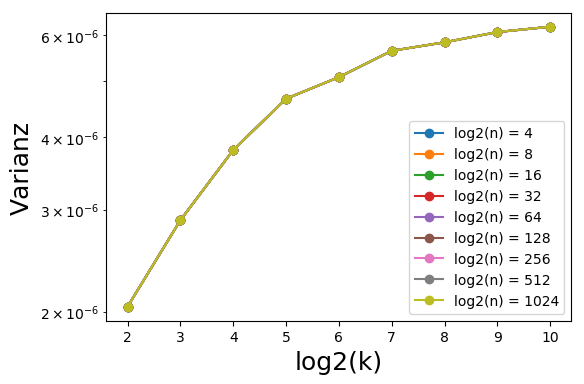
\includegraphics[width=1.21\textwidth]{pictures/min_filter_V_k_log.png}}
    \end{minipage}  
    \hspace*{.8cm}
    \begin{minipage}[t]{.30\textwidth}
        \centering
        \raisebox{0.05cm}{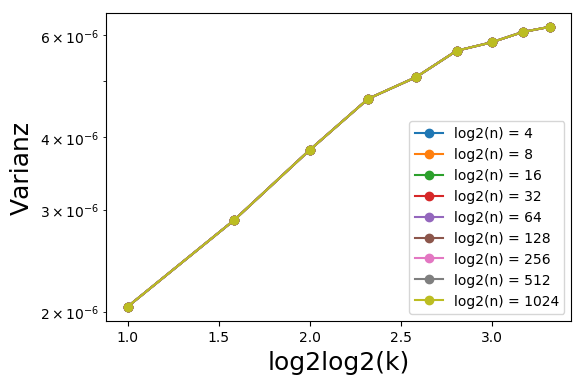
\includegraphics[width=1.21\textwidth]{pictures/min_filter_V_k_loglog.png}}
    \end{minipage}
    \vspace*{-.1cm}
    \captionof{figure}{$V(k)$ für $\log_2(n)=16$ bezüglich $k$, $\log_2(k)$ sowie $\log_2 \log_2(k)$.}\label{fig: min_V_k}
\end{figure}

% ---------------------------------------------------------------
\noindent
Da sich im Verlauf der Experimente eine logarithmischer Zusammenhang erkennen ließ, wurden wie in Abbildung~\ref{fig: min_V_k} zu sehen die Werte von $V(n)$ zuerst gegen die Werte von $k$, dann gegen die logarithmierten und abschließend gegen die doppelt-logarithmierten Werten von $k$ abgetragen. Ist bei der einfach-logarithmischen Darstellung noch eindeutig eine Kurve zu erkennen, so deutet sich bei der doppelt-logarithmischen Darstellung klar ein linearer Funktionsverlauf an.\\[.1cm]
Um sicherzustellen, dass es tatsächlich um einen doppelt-logarithmischen Zusammenhang handelt wurden nun zwei potentielle Fits in Form von $F_V^1(k)= a * \log_2(k) + b$ sowie $F_V^2(k)=a * \log_2\log_2(k) + b$ gebildet. Die nachfolgende Tabelle fasst eine um den Faktor $10^6$ skalierte Gegenüberstellung beider Fits zusammen:

\begin{center}
\begin{tabular}{c||l|l|l|l}

&\multicolumn{1}{c|}{Param $a$}&
\multicolumn{1}{c|}{Param $b$}&
\multicolumn{1}{c|}{Sum Res}&
\multicolumn{1}{c}{$\Delta$ Last Iter}\\
\hline
$F_V^1(k)$:&$0.5212$&$1.5603$&$1.3470$&$-4.6484e-14$\\
\hline
$F_V^2(k)$:&$1.9097$&$0.0636$&$0.1797$&$-9.00343e-10$

\end{tabular}
\end{center}

\noindent
An Parameter $b$ lässt sich bereits erkennen, dass $F_V^1(k)$ eine merkliche Verschiebung auf der $Y$-Achse benötigt, um eine passende Regression zu bilden. Dies sowie die um den Faktor $1.347/0.1797 =7.4958$ höhere Summe der Residuenquadrate legen nahe, dass es sich bei $F_V^2(k)$ um die präzisere Abschätzung handelt, was auch in Abbildung~\ref{fig: min_fit_V_k} noch einmal verdeutlicht wird.

% ---------------------------------------------------------------
%	FIG: Abhängigkeit von K
\begin{figure}[H]
	\hspace*{-1cm}
    \begin{minipage}[t]{.30\textwidth}
        \centering
        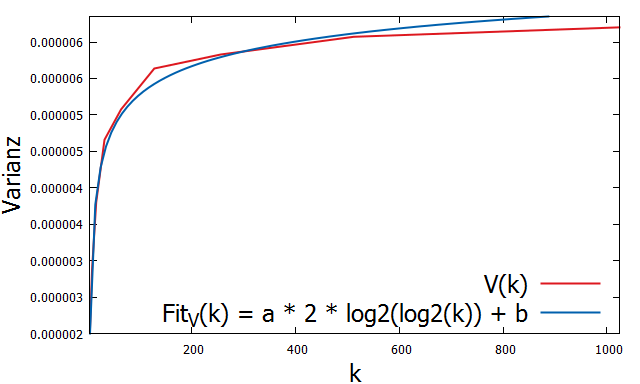
\includegraphics[width=1.2\textwidth]{pictures/min_filter_fit_V_k.png}
    \end{minipage}
    \hspace*{.8cm}
    \begin{minipage}[t]{.30\textwidth}
        \centering
        \raisebox{-0.02cm}{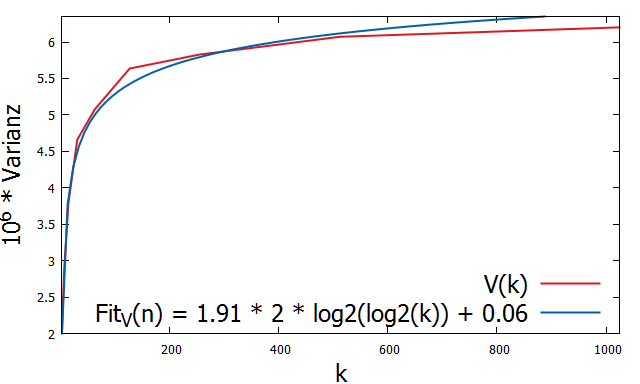
\includegraphics[width=1.21\textwidth]{pictures/min_filter_fit_V_k_loglog.png}}
    \end{minipage}  
    \hspace*{.8cm}
    \begin{minipage}[t]{.30\textwidth}
        \centering
        \raisebox{-0.02cm}{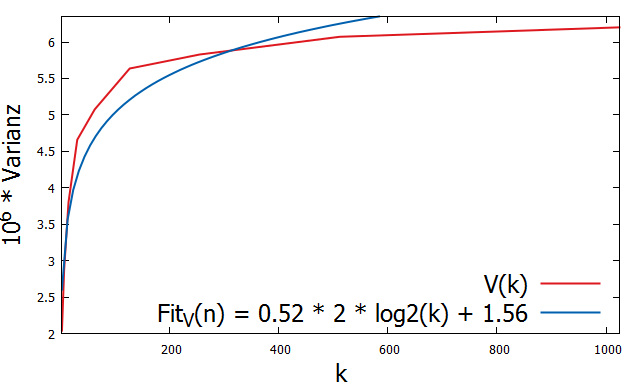
\includegraphics[width=1.21\textwidth]{pictures/min_filter_fit_V_k_log.png}}
    \end{minipage}
    \captionof{figure}{(Skalierter) Fit für $V(k)$ für $\log_2(n)=16$ bezüglich $\log_2(k)$ und $\log_2\log_2(k)$.}\label{fig: min_fit_V_k}
\end{figure}

% ---------------------------------------------------------------
\noindent
Abschließend ist festzuhalten, dass die Güte $\Delta X$ der Filterung einer normalverteilten Zufallsvariable entspricht, deren Erwartungswert von $\sqrt{k}$ und deren Varianz von $1/n$ sowie $\log_2\log_2(k)$ abhängig ist.




%%%%%%%%%%%%%%%%%%%%%%%%%%%%%%%%%%%%%%%%%%%%%%%%%%%%%%%%%%%%%%%%%
%%%%%%%%%%%%%%%%%%%%%%%%%%%%%%%%%%%%%%%%%%%%%%%%%%%%%%%%%%%%%%%%%
\subsubsection{Theorem 4}		%	TESTFÄLLE - RMin
%%%%%%%%%%%%%%%%%%%%%%%%%%%%%%%%%%%%%%%%%%%%%%%%%%%%%%%%%%%%%%%%%

\noindent
Nach Theorem~\ref{theo: min_4} benötigt \Rm $\mathbb{E}[\mfgm]=\mathcal{O}(\varepsilon^{-1}\log\log(n))$ Vergleiche für das Minimum und $\mathbb{E}[\mfgr]=\mathcal{O}(n^{\varepsilon})$ für alle übrigen Elemente.\\[.1cm]
Somit hat die Eingabe nun die Form $(n, n^{\varepsilon})$. Im Folgenden wird zuerst der Parameter $\varepsilon$ und anschließend der Parameter $n$ fixiert, um die Abhängigkeit zu dem jeweils anderen Parameter zu überprüfen.\\
Für die aufgeführten Experimente wurden die Parameter $n$ und $\varepsilon$ so gewählt, dass $n^{\varepsilon}$ weiterhin eine Zweierpotenz ist.\\[.15cm]

\noindent
Nun werden die Auswertungen für $\varepsilon=1/2, 1/4,\gamma$ mit $0<\gamma\ll 1/2$ diskutiert.\\
Es wurden wie auch im Anhang beiliegend weitere Werte durchlaufen, welche jedoch keine nennenswerten Unregelmäßigkeiten aufweisen.\\[.1cm]

%-- HERE
\noindent
Für $\varepsilon=1/2$ wird eine \fg von $\mathbb{E}[\mfgm]=\mathcal{O}(2\cdot\log\log(n))$ für das Minimum und $\mathbb{E}[\mfgr]=\mathcal{O}(n^{1/2})$ für alle übrigen Elemente erwartet.\\
Um diese Aussage zu überprüfen, wurde der Algorithmus nun wiederholt mit dem Eingabetupel $(n', n'^{1/2})$ für die Werte $n'=2^{2\cdot i}$, $i\in \{3,\cdots,20\}$ jeweils Zehntausend mal durchlaufen.
%%%%%%%%%%%%%%%%%%%%%%%%%%%%%%%%%%%%%%%%%%%%%%%%%%%%%%%%%%%%%%%%%
%	MIN
\subsubsection*{\textit{Fragile complexity} des Minimum Elements}
Zuerst untersuchen wir die \fg des Minimums $f_{min}(n)$. 

% ---------------------------------------------------------------
%	FIG: FG Min
\begin{figure}[H]
	\hspace*{-1.1cm}
    \begin{minipage}[t]{.30\textwidth}
        \centering
		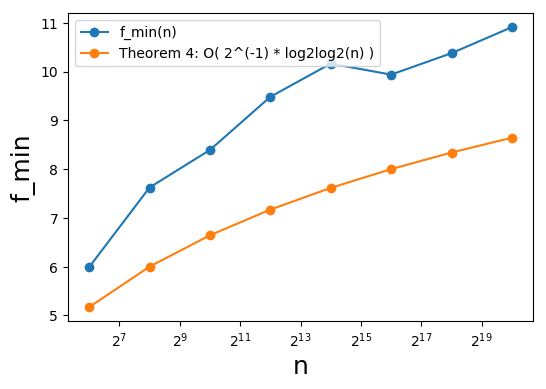
\includegraphics[width=1.075\textwidth]{pictures/min_theo4_2_min_pred.png}
    \end{minipage}
    \hspace*{0.4cm}
    \begin{minipage}[t]{.30\textwidth}
        \centering
        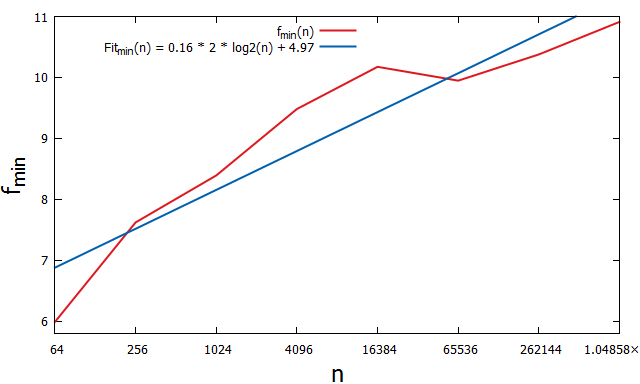
\includegraphics[width=1.21\textwidth]{pictures/min_theo4_2_fit_min_log.png}
    \end{minipage}
    %
    \hspace*{0.85cm}
	%    
    \begin{minipage}[t]{.30\textwidth}
        \centering
        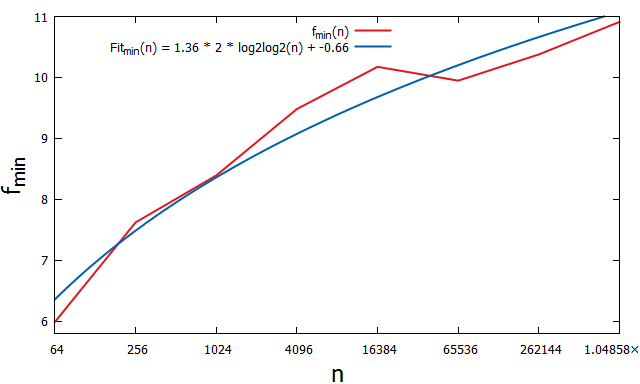
\includegraphics[width=1.21\textwidth]{pictures/min_theo4_2_fit_min_loglog.png}
    \end{minipage}
    \vspace*{-.1cm}
    \captionof{figure}{(Skalierter) Vorhersage und Fit für $f_{min}(n)$ mit $k(n)=n^{1/2}$.}\label{fig: min_theo4_fit_min}
\end{figure}

% ---------------------------------------------------------------
\noindent
Wie im ersten Bild der Abbildung~\ref{fig: min_theo4_fit_min} zu sehen wurde die aus Theorem~\ref{theo: min_4} stammende Abschätzung ohne weitere Parametrisierung in ein Koordinatensystem eingetragen. Abgesehen von einer leichten Verschiebung stimmen die Bilder der Funktionen gut überein. Im mittleren Bild wird eine einfach-logarithmischer Abschätzung dargestellt. Wie jedoch nach dem logarithmischen Skalieren der $X$-Achse zu sehen ist, weist $f_{min}(n)$ weiterhin eine kurvenförmige Darstellung auf, womit der einfach-logarithmische Fall nahezu ausgeschlossen werden kann.\\[.1cm]
In der Praxis wurde sowohl ein Fit der Form $F_{min}^1(n)= a \cdot \varepsilon^{-1}\cdot \log_2(n) + b = a \cdot 2\cdot\log_2(n) + b$ als auch ein Fit der Form $F_{min}^1(n)= a \cdot 2\cdot\log_2\log_2(n) + b$ mit Startwerten $a=1$ und $b=0.001$ versucht. Es ergab sich folgende Gegenüberstellung beider Fits:

\begin{center}
\begin{tabular}{c||l|l|l|l}

&\multicolumn{1}{c|}{Param $a$}&
\multicolumn{1}{c|}{Param $b$}&
\multicolumn{1}{c|}{Sum Res}&
\multicolumn{1}{c}{$\Delta$ Last Iter}\\
\hline
$F_V^1(k)$:&$0.1595$&$4.9664$&$2.1959$&$-2.03746e-09$\\
\hline
$F_V^2(k)$:&$1.3571$&$-0.6563$&$0.7404$&$-1.34947e-13$

\end{tabular}
\end{center}

\noindent
Die Tatsache, dass der Parameter $b$ im einfach-logarithmischen Fall um den Faktor $7.57$ weiter von $0$ entfernt konvergiert ist als der doppelt-logarithmische, zusammen mit der deutlich höheren Summe der Residuenquadrate lassen den Schluss zu, dass die Vorhersage des Theorems für die \fg des Minimums \fgm auch in der Praxis bestätigt werden kann.

%%%%%%%%%%%%%%%%%%%%%%%%%%%%%%%%%%%%%%%%%%%%%%%%%%%%%%%%%%%%%%%%%
%	Rem
\subsubsection*{\textit{Fragile complexity} aller nicht-Minimum Elemente}
Nun wird die \fg aller übrigen Elemente $f_{rem}(n)$ untersucht. Theorem~\ref{theo: min_4} prognostiziert in diesem Fall eine \fg von $\mO(n^{\varepsilon})$. Vergleicht man die experimentell gemessenen Werte für  $f_{rem}(n)$ mit dem Term $n^{\varepsilon}$ bei gleicher Parametrisierung, so ergibt sich eine nahezu perfekte Übereinstimmung. Aus diesem Grund wurde in diesem Fall auf einen Fit verzichtet.\\[.1cm]

\noindent
Wie in Abbildung~\ref{fig: min_theo4_fit_rem} ebenfalls zu sehen wird die in Theorem~\ref{theo: min_3} prognostizierte Linearität der Arbeit $w(n)$ exakt eingehalten. Abschließend sei noch bemerkt, dass der Algorithmus erst ab einer Mächtigkeit der Eingabemenge $\log_2(n)=10$ den ersten rekursiven Aufruf tätigt.


% ---------------------------------------------------------------
%	FIG: FG Min
\begin{figure}[H]
	\hspace*{-1.1cm}
    \begin{minipage}[t]{.30\textwidth}
        \centering
        \raisebox{0.05cm}{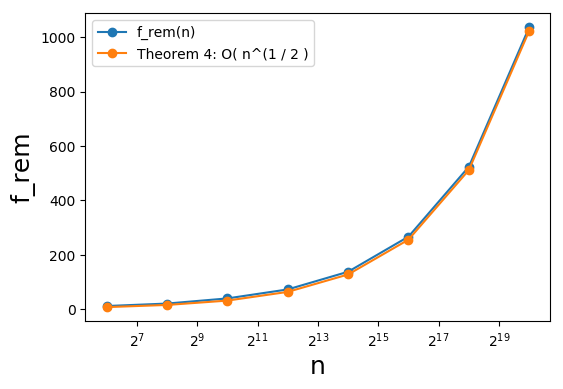
\includegraphics[width=1.21\textwidth]{pictures/min_theo4_2_rem_pred.png}
        \vspace*{.05cm}}
    \end{minipage}
    \hspace*{.8cm}
    \begin{minipage}[t]{.30\textwidth}
        \centering
        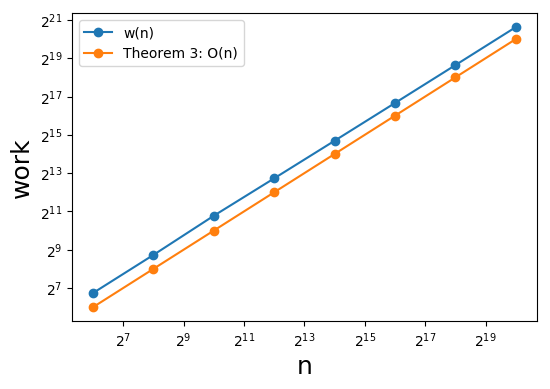
\includegraphics[width=1.2\textwidth]{pictures/min_theo4_2_work.png}
    \end{minipage}
    \hspace*{.8cm}
    \begin{minipage}[t]{.30\textwidth}
        \centering
        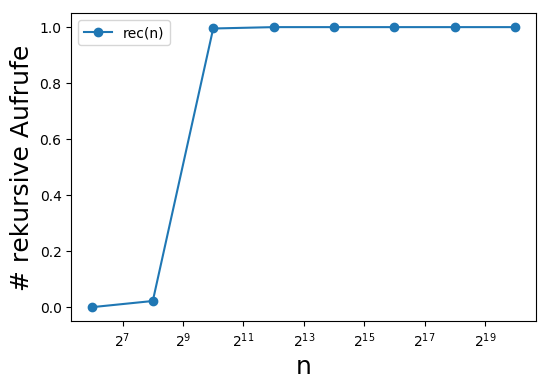
\includegraphics[width=1.21\textwidth]{pictures/min_theo4_2_rec.png}
    \end{minipage}
    \vspace*{-.1cm}
    \captionof{figure}{Vorhersage für $f_{rem}(n)$, $w(n)$ und $rec(n)$ mit $k(n)=n^{1/2}$.}\label{fig: min_theo4_fit_rem}
\end{figure}


%%%%%%%%%%%%%%%%%%%%%%%%%%%%%%%%%%%%%%%%%%%%%%%%%%%%%%%%%%%%%%%%%
%%%%%%%%%%%%%%%%%%%%%%%%%%%%%%%%%%%%%%%%%%%%%%%%%%%%%%%%%%%%%%%%%
\subsubsection{Theorem 5}		%	TESTFÄLLE - RMin
%%%%%%%%%%%%%%%%%%%%%%%%%%%%%%%%%%%%%%%%%%%%%%%%%%%%%%%%%%%%%%%%%

\noindent
Nach Theorem~\ref{theo: min_5} benötigt \Rm $\mathbb{E}[\mfgm]=\mathcal{O}(\varepsilon^{-1}\log\log(n))$ Vergleiche für das Minimum und $\mathbb{E}[\mfgr]=\mathcal{O}(n^{\varepsilon})$ für alle übrigen Elemente.\\[.1cm]
Da $k(n)$ bei der Eingabe ganzzahlig sein muss, wurde der Wert vor der Eingabe sowohl auf- als auch abgerundet und beide Fälle separat betrachtet. Wie zuvor wird für beide Fälle einen passenden Fit $F_{\lceil k \rceil}(n)$ beziehungsweise $F_{\lfloor k \rfloor}(n)$ untersucht. Für eine präzisere Repräsentation des Parameters $k(n)$ wird zusätzlich ein weiter Fit mit folgender Gewichtung gebildet:
\[F^{\star}(n) = (\lceil k \rceil - k) \cdot f_{\lfloor k\rfloor}(n) + (k - \lfloor k \rfloor)\cdot f_{\lceil k \rceil}(n)
\]\label{other: weigh}

\noindent
Hierbei werden die auf- und abgerundeten Werte relativ entsprechend ihrer absoluten Differenz von dem realen Wert des Parameters $k(n)$ gewichtet. Die Repräsentation für Theorem~\ref{theo: min_5} beruht auf Eingaben für $\log_2(n)=\{6,\cdots,20\}$, mit denen wie zuvor zuerst die \fg des Minimums \fgm und dann die aller übrigen Elemente \fgr experimentell analysiert werden.

%%%%%%%%%%%%%%%%%%%%%%%%%%%%%%%%%%%%%%%%%%%%%%%%%%%%%%%%%%%%%%%%%
%	FRAGILE COMPLEXITY - MINIMUM
\subsubsection*{\textit{Fragile complexity} des Minimum Elements}
Nun wird die Aussage von Theorem~\ref{theo: min_5} bezüglich der \fg des Minimums \fgm untersucht. Es wurden nun wie besprochen drei separate Fits bezüglich der entsprechend gesammelten Datenmenge gebildet. Bei einer Wahl der Startwerte von $a=5$, $b=0.001$ ist der Fit nach $8$, für $a=6.5$, $b=-8.5$ nach $4$ Iteration konvergiert und es ergab sich in beiden Fällen:
\begin{center}
\begin{tabular}{c||l|l|l|l}

&\multicolumn{1}{c|}{Param $a$}&
\multicolumn{1}{c|}{Param $b$}&
\multicolumn{1}{c|}{Sum Res}&
\multicolumn{1}{c}{$\Delta$ Last Iter}\\
\hline
$F_{\lceil k \rceil}(n)$:&$6.97$&$-9.91$&$0.4546$&$-3.23746e-09$\\
\hline
$F_{\lfloor k \rfloor}(n)$:&$6.42$&$-7.88$&$2.2034$&$-4.2210e-13$\\
\hline
$F^{\star}(n)$:&$6.66$&$-8.78$&$1.3096$&$-8.8166e-10$
\end{tabular}
\end{center}

\noindent
Wie zu erkennen, ist die sich ergebende Parametrisierung von $a$ und $b$ in allen Fällen relativ ähnlich. Die Parameter fallen für $F_{\lfloor k \rfloor}(n)$ am geringsten aus, jedoch ist die Summe der Residuenquadrate hier auch am Höchsten.\\[.1cm]
Wie in Abbildung~\ref{fig: min_theo5_fit_min} zu sehen, weicht die gesammelte Datenmenge vorerst leicht von der Prognose des Theorems ab. Skaliert man diese jedoch entsprechend des errechneten Fits, so ergibt sich eine beinahe deckungsgleiche Darstellung zu der gesammelten Datenmenge. Der Fit ist so eindeutig, dass auf eine einfach-logarithmische Abschätzung als Vergleich verzichtet wurde.

% ---------------------------------------------------------------
%	FIG: FG Min
\begin{figure}[H]
	\hspace*{-.4cm}
    \begin{minipage}[t]{.30\textwidth}
        \centering
        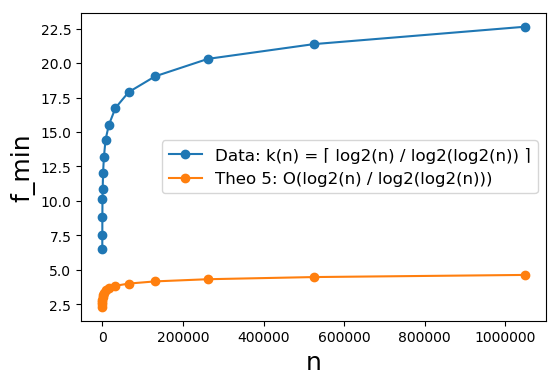
\includegraphics[width=1.1\textwidth]{pictures/min_theo5_min_ceil_pred.png}
        \vspace*{-0.06cm}
    \end{minipage}
    \hspace*{.4cm}
    \begin{minipage}[t]{.30\textwidth}
        \centering
        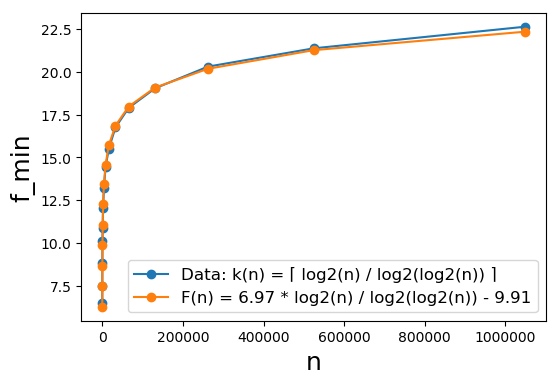
\includegraphics[width=1.11\textwidth]{pictures/min_theo5_min_ceil_fit.png}
    \end{minipage}
    \hspace*{.4cm}
    \begin{minipage}[t]{.30\textwidth}
        \centering
        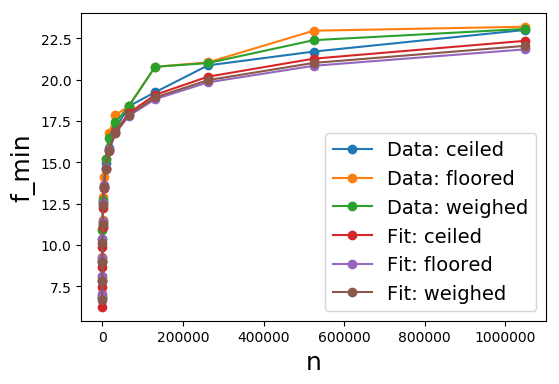
\includegraphics[width=1.11\textwidth]{pictures/min_theo5_min_all.png}
    \end{minipage}
    \vspace*{-0.1cm}
    \captionof{figure}{Vorhersage und Fit für \fgm bezüglich Auf- und Abrundung.}\label{fig: min_theo5_fit_min}
\end{figure}

% ---------------------------------------------------------------
\noindent
Dies lässt die Aussage von Theorem~\ref{theo: min_5} bezüglich der \fg des Minimums \fgm eindeutig bestätigen.

\subsubsection*{\textit{Fragile complexity} aller nicht-Minimum Elemente}
Nun wird eine analoge Betrachtung bezüglich der \fg aller übrigen Elemente $f_{rem}(n)$ durchgeführt. Die Prognose von Theorem~\ref{theo: min_5} bezüglich der \fg ist identisch für das Minimum und für alle übrigen Elemente. Das Ergebnis für \fgr weist keine Unregelmäßigkeiten auf und es bilden sich ähnliche Abschätzungen wie bereits für $f_{min}(n)$:

\begin{center}
\begin{tabular}{c||l|l|l|l}

&\multicolumn{1}{c|}{Param $a$}&
\multicolumn{1}{c|}{Param $b$}&
\multicolumn{1}{c|}{Sum Res}&
\multicolumn{1}{c}{$\Delta$ Last Iter}\\
\hline
$F_{\lceil k \rceil}(n)$:&$7.14$&$-10.38$&$0.8468$&$-7.22016e-09$\\
\hline
$F_{\lfloor k \rfloor}(n)$:&$7.44$&$-10.96$&$2.0026$&$-8.9850e-10$\\
\hline
$F^{\star}(n)$:&$7.37$&$-10.88$&$1.8968$&$-9.3543e-10$
\end{tabular}
\end{center}

\noindent
Abschließend sei hier noch anzumerken, dass die für diese Eingabe von \Rm benötigte Arbeit $w(n)$ mit wachsendem $n$ linear skaliert. Somit kann die Aussage von Theorem~\ref{theo: min_3} weiterhin bestärkt werden und neben einer Darstellung des Fits für \fgr abschließend in Abbildung~\ref{fig: min_theo5_fit_rem} eingesehen werden. 

% ---------------------------------------------------------------
%	FIG: FG Min
\begin{figure}[H]
	\hspace*{-1.1cm}
    \begin{minipage}[t]{.30\textwidth}
        \centering
        \raisebox{0.05cm}{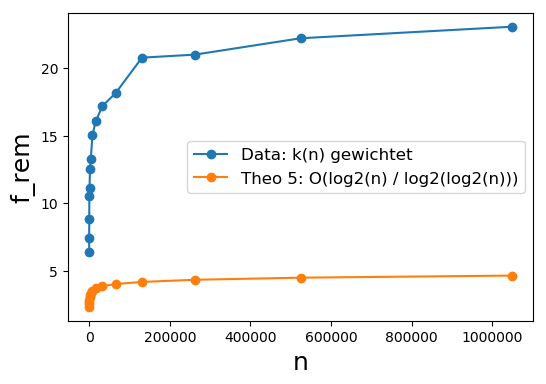
\includegraphics[width=1.15\textwidth]{pictures/min_theo5_rem_weigh_pred.png}}
    \end{minipage}
    \hspace*{.6cm}
    \begin{minipage}[t]{.30\textwidth}
        \centering
        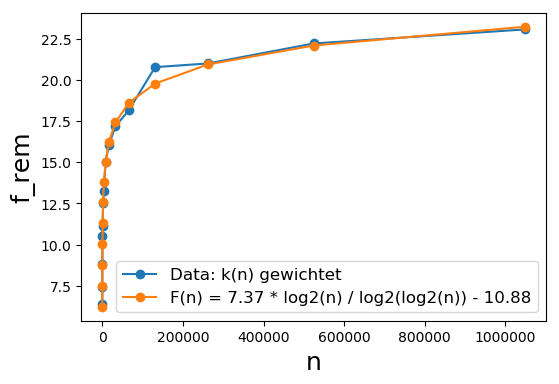
\includegraphics[width=1.2\textwidth]{pictures/min_theo5_rem_weigh_fit.png}
    \end{minipage}
    \hspace*{.8cm}
    \begin{minipage}[t]{.30\textwidth}
        \centering
        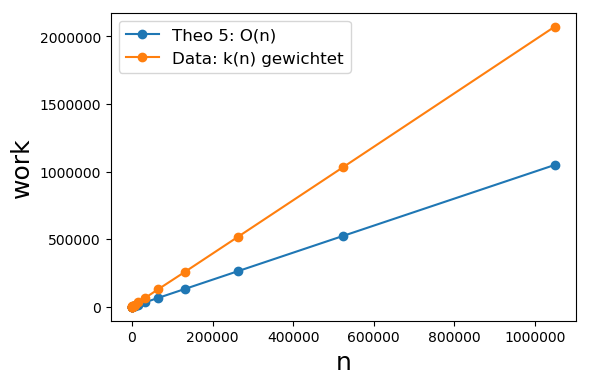
\includegraphics[width=1.25\textwidth]{pictures/min_theo5_work_weigh_pred.png}
    \end{minipage}
    \vspace*{-0.1cm}
    \captionof{figure}{Vorhersage und Fit für \fgr sowie die Arbeit $w(n)$.}\label{fig: min_theo5_fit_rem}
\end{figure}

% ---------------------------------------------------------------
\noindent
Dies beendet die experimentelle Analyse dieser Arbeit bezüglich des in Paper~\cite{meyer1} vorgestellten Algorithmus \Rm und der \fg des Minimums sowie aller übrigen Elemente.\\[.1cm]
Es konnte ein Zusammenhang zwischen den Eingabeparametern $n$ und $k(n)$ sowie der Güte der Filterung der ersten drei Phasen nachgewiesen, sowie die Aussagen der Theoreme 3-5 des Papers eindeutig bekräftigt werden.\\[.1cm]
Weitere untersuchte Fälle liegen der Arbeit bei und können zusätzlich im Anhang nachgeschlagen werden. 

%%%%%%%%%%%%%%%%%%%%%%%%%%%%%%%%%%%%%%%%%%%%%%%%%%%%%%%%%%%%%%%%%
%%%%%%%%%%%%%%%%%%%%%%%%%%%%%%%%%%%%%%%%%%%%%%%%%%%%%%%%%%%%%%%%%
\subsection{\RM}		%	TESTFÄLLE - RMed
%%%%%%%%%%%%%%%%%%%%%%%%%%%%%%%%%%%%%%%%%%%%%%%%%%%%%%%%%%%%%%%%%

\noindent
Nun wird eine vergleichbare Analyse für den Algorithmus \RM durchgeführt. Hierbei wird die Güte der Approximation der Theoreme~\ref{theo: med_28} und ~\ref{theo: med_29} aus dem Paper~\cite[S.24]{meyer2} experimentell untersucht.\\[.1cm]
Aufgrund der limitierten Zeit dieser Arbeit und der im direkten Vergleich zu \Rm deutlich höheren Laufzeit, konnte der Datensatz für den Algorithmus \RM nicht so umfangreich ausfallen wie gehofft. Die vorliegende Implementierung erlaubt diesen jedoch nach Bedarf aufzustocken. Wie bei seiner Analyse bereits festgehalten wurde, ist die Auswertung des Algorithmus \RM für eine Eingabemenge $X$ mit einer Mächtigkeit von $n \leq 2^{16}$ uninteressant. Somit wurden für den Parameter $n$ die Werte $n =2^i$, $i\in\{16,\cdots,20\}$ gewählt.\\[.05cm]
Um jedoch ein Gefühl für die Auswirkung der Parameter zu gewinnen wurde zum Test der Parameter $d(n)$ auf die nächst größere beziehungsweise kleinere Ganzzahl gerundet. Bei der Wahl von $n=2^{18}$, $k(n)=2^{12}$ sowie $d_1(n)=2$ und $d_2(n)=3$ halbiert sich, wie in Abbildung~\ref{fig: med_theo28_comp} zu sehen, sowohl die \fg des Median Elements, als auch die Arbeit $w(n)$ bei Auf- und Abrundung zwischen $2$ und $3$. Die \fg aller nicht-Median Elemente \fgr verdoppelt sich hingegen.

% ---------------------------------------------------------------
%	FIG: FG COMP
\begin{figure}[H]
	\hspace*{-1.1cm}
    \begin{minipage}[t]{.30\textwidth}
        \centering
		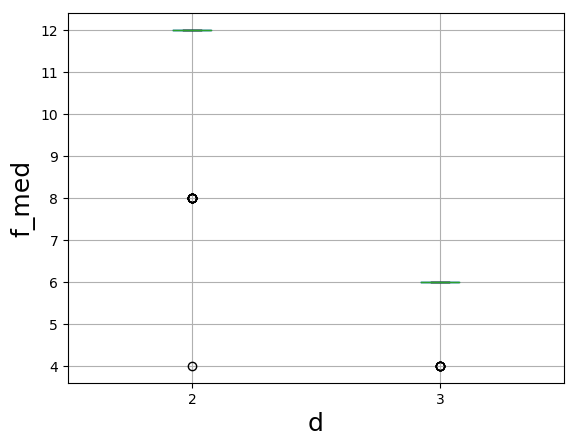
\includegraphics[width=1.15\textwidth]{pictures/med_algo_theo28_comp_med}
    \end{minipage}
    \hspace*{.6cm}
    \begin{minipage}[t]{.30\textwidth}
        \centering
        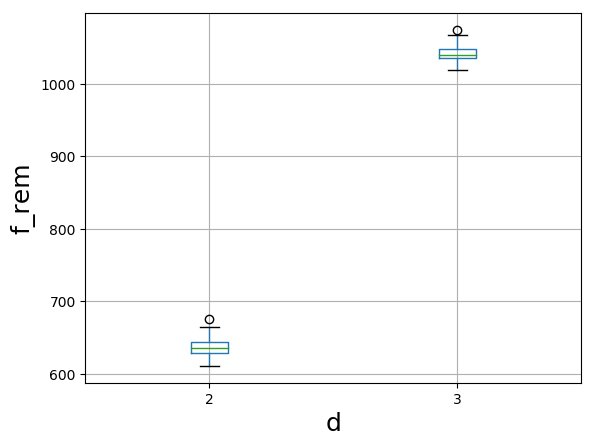
\includegraphics[width=1.2\textwidth]{pictures/med_algo_theo28_comp_rem}
    \end{minipage}
    \hspace*{.8cm}
    \begin{minipage}[t]{.30\textwidth}
        \centering
        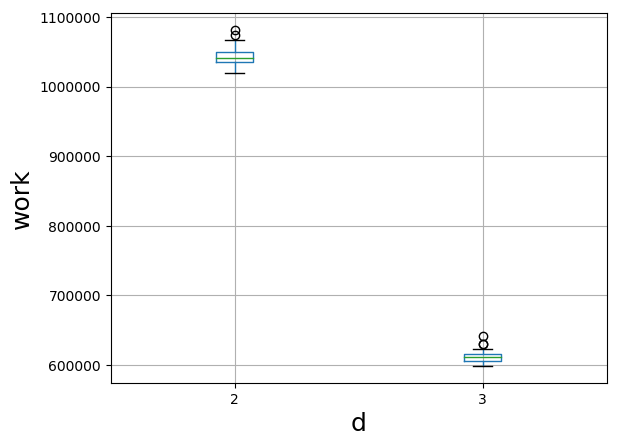
\includegraphics[width=1.25\textwidth]{pictures/med_algo_theo28_comp_work.png}
    \end{minipage}
    \vspace*{-0.1cm}
    \captionof{figure}{Vorhersage und Fit für \fgr sowie die Arbeit $w(n)$.}\label{fig: med_theo28_comp}
\end{figure}

\noindent
Somit ergibt sich ein merklicher Sprung für die \fg aller Elemente, sobald $d(n)$ die nächste Ganzzahl überschreitet. Dies hat direkte Konsequenzen für die Analyse dieser Arbeit, da für die notwendige Parametrisierung nach Theorem~\ref{theo: med_28} bei $k(2^{18}) <3$ sowie $k(2^{19}) \geq 3$ gilt, was das Ergebnis einer Regression verzerrt. Für zukünftige Forschungen wäre es interessant, den Parameter $d(n)$ speziell zu gewichten oder auf bestimmten Intervallen gesondert zu betrachten, was im Rahmen dieser Arbeit zeitlich nicht mehr realisierbar war.
%%%%%%%%%%%%%%%%%%%%%%%%%%%%%%%%%%%%%%%%%%%%%%%%%%%%%%%%%%%%%%%%%

%%%%%%%%%%%%%%%%%%%%%%%%%%%%%%%%%%%%%%%%%%%%%%%%%%%%%%%%%%%%%%%%%
\subsubsection{Theorem 28}		%	TESTFÄLLE - RMed - Theorem 28
%%%%%%%%%%%%%%%%%%%%%%%%%%%%%%%%%%%%%%%%%%%%%%%%%%%%%%%%%%%%%%%%%

\noindent
Nach Theorem~\ref{theo: med_28} des Papers~\cite{meyer2} erreicht das Median Element für $k(n)=n^{2/3}$ und $d(n)=n^{1/12}$ eine erwartete \fg von $\mathbb{E}[f_{med}(n)]=\mO(\log\log(n))$ und alle übrigen Elemente $\mathbb{E}[f_{rem}(n)]=\mO(\sqrt{n})$.\\[.1cm]





\subsubsection*{\textit{Fragile complexity} des Median Elements}
Zuerst wird die \fg des Medians \fgM untersucht. Wie bereits erwähnt findet ein die Werte verzerrender Sprung statt, wie in Abbildung~\ref{fig: med_theo28_work} deutlich zu sehen. Die Arbeit $w(n)$ verhält sich jedoch wie erwartet linear, was Theorem~\ref{theo: med_30} bestätigt.

%---------------------------------------------------------------
%	FIG: FG COMP
\begin{figure}[H]
	\hspace*{-.6cm}
    \begin{minipage}[t]{.30\textwidth}
        \centering
		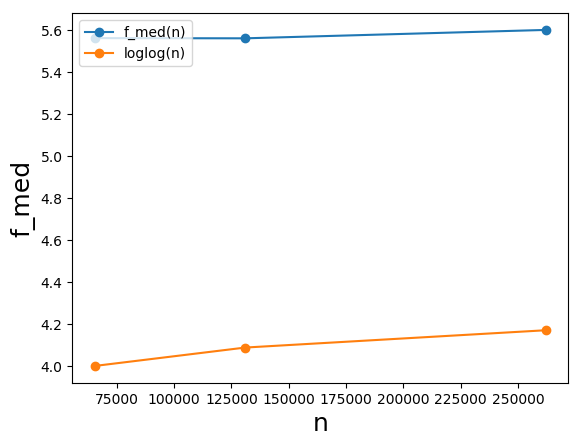
\includegraphics[width=\textwidth]{pictures/med_algo_theo28_med}
    \end{minipage}
    \hspace*{.4cm}
    \begin{minipage}[t]{.30\textwidth}
        \centering
        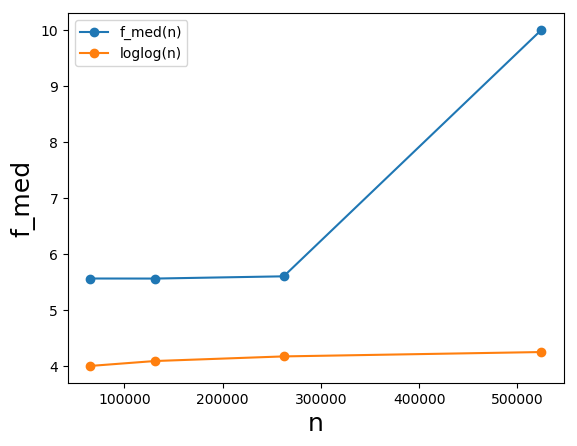
\includegraphics[width=\textwidth]{pictures/med_algo_theo28_med_jump}
    \end{minipage}
    \hspace*{.4cm}
    \begin{minipage}[t]{.30\textwidth}
        \centering
        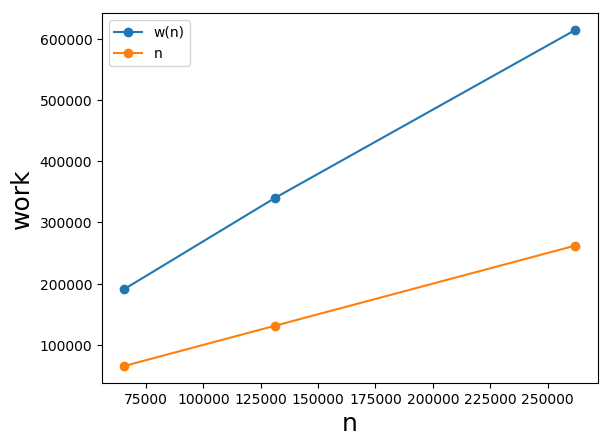
\includegraphics[width=\textwidth]{pictures/med_algo_theo28_work.png}
    \end{minipage}
    \vspace*{-0.1cm}
    \captionof{figure}{$\log(n)=16,\cdots,18$ gegenüber $\log(n)=16,\cdots,19$ sowie die Arbeit $w(n)$.}\label{fig: med_theo28_work}
\end{figure}


%---------------------------------------------------------------
\noindent
Auch wenn die Datenmenge sowie der gesammelte Bereich nicht ausreichen, um eine feste Aussage zu tätigen, wurde die \fg trotzdem für $\log(n)=16,\cdots,18$ untersucht. Die Daten wurden hierbei wieder gegen einen einfach-logarithmischen mit $F^1(n)=a\cdot\log(n) + b$ sowie eine doppelt-logarithmischen Term $F^2(n)=a\cdot\log\log(n) + b$ abgeglichen.

\begin{center}
\begin{tabular}{c||l|l|l|l}

&\multicolumn{1}{c|}{Param $a$}&
\multicolumn{1}{c|}{Param $b$}&
\multicolumn{1}{c|}{Sum Res}&
\multicolumn{1}{c}{$\Delta$ Last Iter}\\
\hline
$F^1(n)$:&$0.2272$&$4.6452$&$0.0002$&$-2.42876e-07$\\
\hline
$F^2(n)$:&$0.0195$&$5.2419$&$0.0002$&$-1.9372e-14
$
\end{tabular}
\end{center}
Die sich ergebenden experimentellen Daten sowie ihre grafische Veranschaulichung in Abbildung~\ref{fig: med_theo28_med} deuten stark auf einen, wie von Theorem~\ref{theo: med_28} angegebenen, doppelt-logarithmischen Zusammenhang hin. Eine logarithmische Achsenskalierung hilft hier jedoch nicht, um eine Abschätzung jeglicher Form zu unterstützen. 


%---------------------------------------------------------------
%	FIG: FG COMP
\begin{figure}[H]
	\hspace*{-0.4cm}
    \begin{minipage}[t]{.30\textwidth}
        \centering
		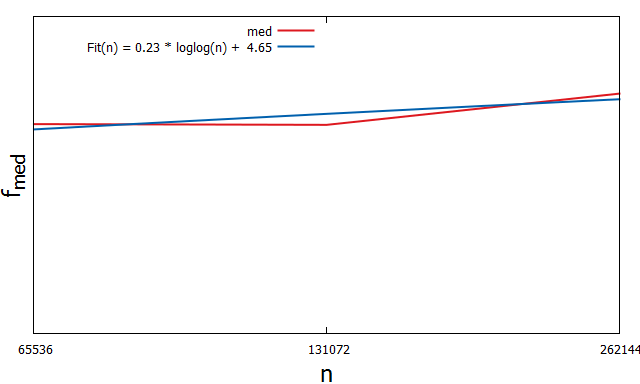
\includegraphics[width=1.15\textwidth]{pictures/med_algo_theo28_fit_med_loglog}
    \end{minipage}
    \hspace*{.6cm}
    \begin{minipage}[t]{.30\textwidth}
        \centering
        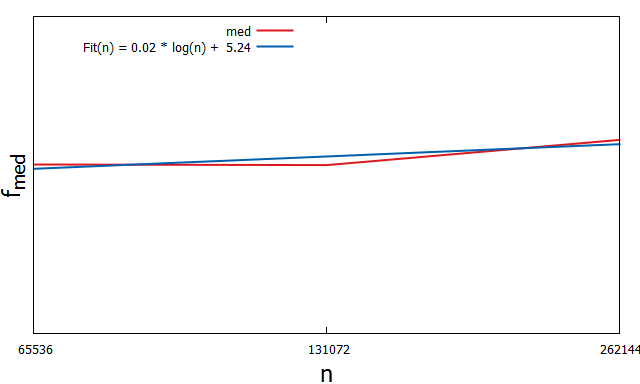
\includegraphics[width=1.15\textwidth]{pictures/med_algo_theo28_fit_med_log}
    \end{minipage}
    \hspace*{.8cm}
    \begin{minipage}[t]{.30\textwidth}
        \centering
        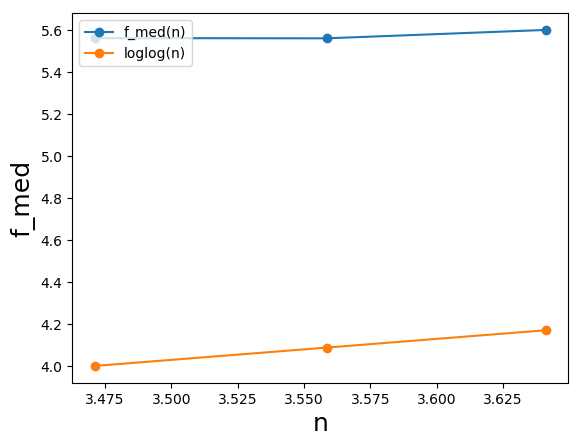
\includegraphics[width=\textwidth]{pictures/med_algo_theo28_med_logscale.png}
    \end{minipage}
    \vspace*{-0.1cm}
    \captionof{figure}{$\log$ vs $\log\log$ Fit sowie logarithmische Achsenskalierung.}\label{fig: med_theo28_med}
\end{figure}


%---------------------------------------------------------------
\noindent

\subsubsection*{\textit{Fragile complexity} aller nicht-Median Elemente}
Für die \fg aller nicht-Median Elemente \fgr hingegen konnte eine aussagekräftige Regression gewonnen werden.\\[.05cm]
Wie in Abbildung~\ref{fig: med_theo28_rem} zu sehen wurde hier ein Fit der Form $F(n)= a \cdot \sqrt{n} + b$ mit einer Parametrisierung von $a=2.3374$  $b=-155.424$ bestimmt.


%---------------------------------------------------------------
%	FIG: FG COMP
\begin{figure}[H]
	\hspace*{-.8cm}
    \begin{minipage}[t]{.30\textwidth}
        \centering
		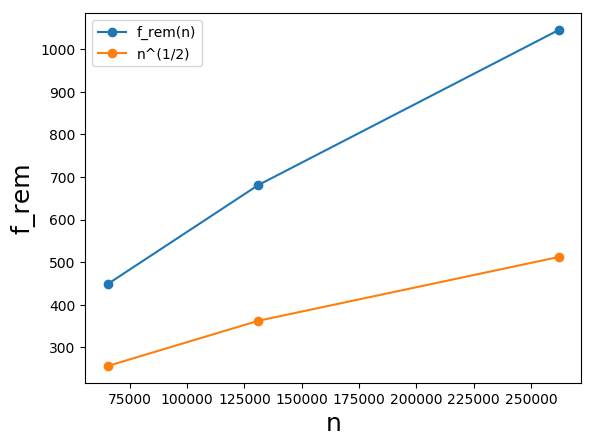
\includegraphics[width=\textwidth]{pictures/med_algo_theo28_rem}
    \end{minipage}
    \hspace*{.3cm}
    \begin{minipage}[t]{.30\textwidth}
        \centering
        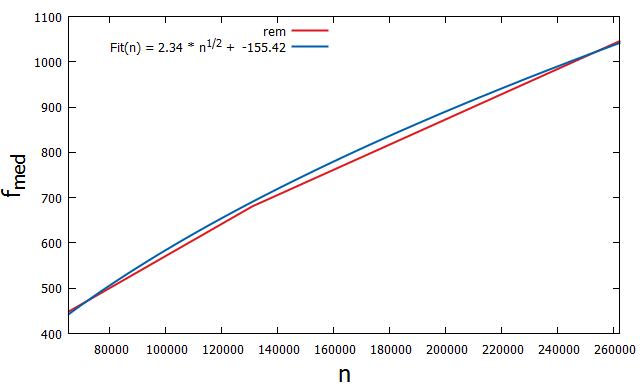
\includegraphics[width=1.25\textwidth]{pictures/med_algo_theo28_fit_rem}
    \end{minipage}
    \hspace*{1.2cm}
    \begin{minipage}[t]{.30\textwidth}
        \centering
        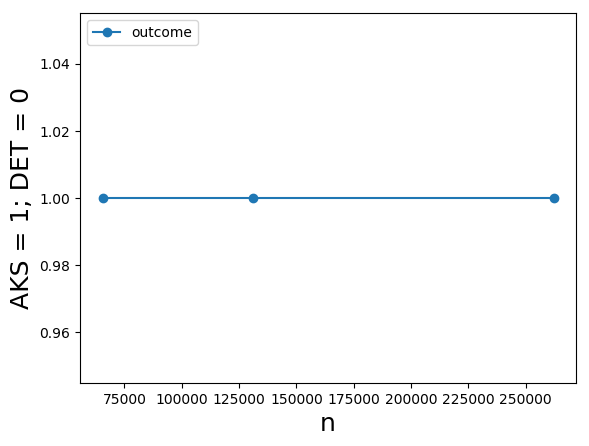
\includegraphics[width=\textwidth]{pictures/med_algo_theo28_case.png}
    \end{minipage}
    \vspace*{-0.1cm}
    \captionof{figure}{Vorhersage und Fit für \fgr sowie der Ausgang von Phase 3.}\label{fig: med_theo28_rem}
\end{figure}


%---------------------------------------------------------------
\noindent
Abschließend sei hier noch angemerkt, dass bei allen für die Grafiken genutzten Experimentaldaten der Algorithmus \RM mit der Ausführung des \textit{AKS}-Algorithmus endet.





%%%%%%%%%%%%%%%%%%%%%%%%%%%%%%%%%%%%%%%%%%%%%%%%%%%%%%%%%%%%%%%%%
\subsubsection{Theorem 29}		%	TESTFÄLLE - RMed - Theorem 29
%%%%%%%%%%%%%%%%%%%%%%%%%%%%%%%%%%%%%%%%%%%%%%%%%%%%%%%%%%%%%%%%%

\noindent
Nach Theorem~\ref{theo: med_29} des Papers~\cite{meyer2} erreicht das Median Element für $k(n)=n / \log^{1/3}(n)$ und $d(n)=\log^{1/3}(n)$ eine erwartete \fg von $\mathbb{E}[f_{med}(n)]=\mO(\log\log(n))$ und alle übrigen Elemente eine erwartete \fg von $\mathbb{E}[f_{rem}(n)]=\mO(\sqrt{n})$.\\[.05cm]

\subsubsection*{\textit{Fragile complexity} des Median Elements}
Für die \fg des Medians \fgm lässt sich die Schranke aus Theorem~\ref{theo: med_29} trotz beschränkter Datenmenge eindeutig bestätigen.\\[.05cm]
In Abbildung~\ref{fig: med_theo29_med} zu sehen erkennt man schon bei direktem Vergleich zwischen den Experimentaldaten und der Funktion $f(x)=\log(x)$ der Daten die bestehende Korrelation. Parametrisiert man diese über einen Fit der Form $F(x)=a\cdot \log(x) + b$, so wie zu erkennen eine gute Übereinstimmung.

%---------------------------------------------------------------
%	FIG: FG COMP
\begin{figure}[H]
	\hspace*{-.9cm}
    \begin{minipage}[t]{.30\textwidth}
        \centering
		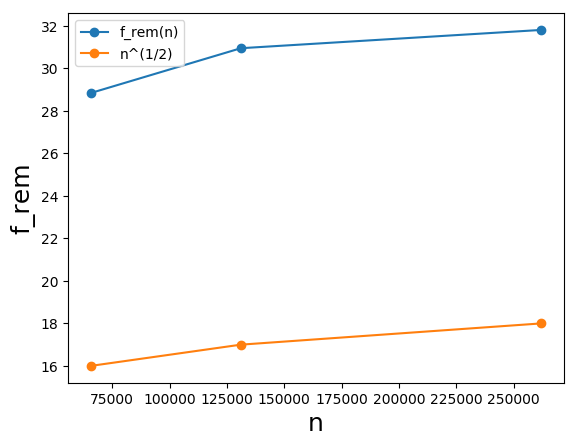
\includegraphics[width=0.95\textwidth]{pictures/med_algo_theo29_rem}
    \end{minipage}
    \hspace*{.3cm}
    \begin{minipage}[t]{.30\textwidth}
        \centering
        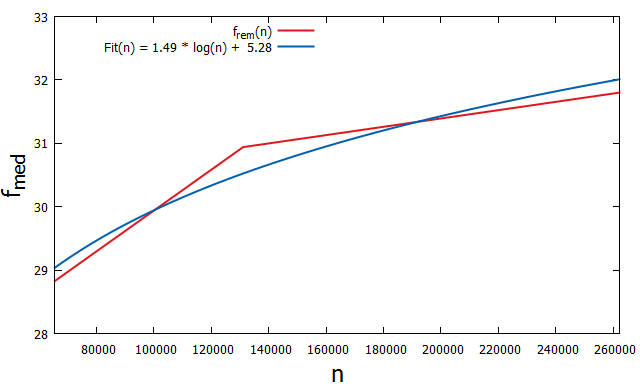
\includegraphics[width=1.25\textwidth]{pictures/med_algo_theo29_fit_rem}
    \end{minipage}
    \hspace*{1.2cm}
    \begin{minipage}[t]{.30\textwidth}
        \centering
        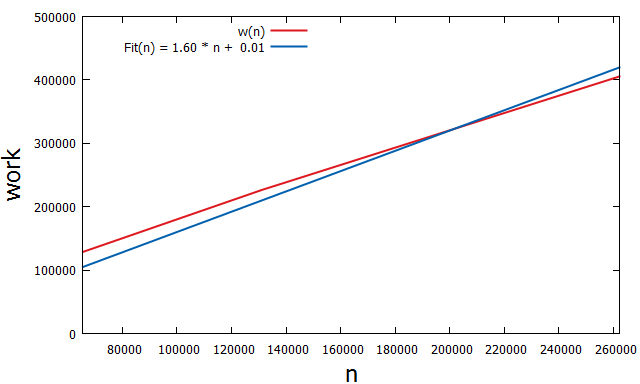
\includegraphics[width=1.25\textwidth]{pictures/med_algo_theo29_fit_work.png}
    \end{minipage}
    \vspace*{-0.1cm}
    \captionof{figure}{Vorhersage und Fit für \fgr sowie die Arbeit $w(n)$.}\label{fig: med_theo29_med}
\end{figure}

\noindent
Auch bei einer Parametrisierung nach Theorem~\ref{theo: med_29} wurde der Algorithmus \RM stets durch den \textit{AKS}-Algorithmus beendet. Um eine Abschätzung für die Wahrscheinlichkeit einer unglücklichen Wahl eines Samples der ersten Phase des Algorithmus zu liefern bedarf es einer deutlich umfangreicheren Datenmenge, so dass im Rahmen dieser Arbeit diesbezüglich keine Aussage getroffen werden kann. 


\subsubsection*{\textit{Fragile complexity} aller nicht-Median Elemente}
Abschließend untersuchen wir noch die \fg aller nicht-Median Elemente \fgr sowie die von dem Algorithmus \RM verrichtete Arbeit $w(n)$.\\[.05cm]
Wie in Abbildung~\ref{fig: med_theo29_rem} zu sehen ist bereits eine direkte Ähnlichkeit zwischen den Experimentaldaten und der Funktion $f(x)=\log(x)$ erkennbar. Wie zu erwarten konnte ein passender Fit der Form $F(n)= a\cdot \log(n) +b$ mit Parametern $a=1.49$ und $b=5.28$ berechnet werden.
%---------------------------------------------------------------
%	FIG: FG COMP
\begin{figure}[H]
	\hspace*{-0.9cm}
    \begin{minipage}[t]{.30\textwidth}
        \centering
		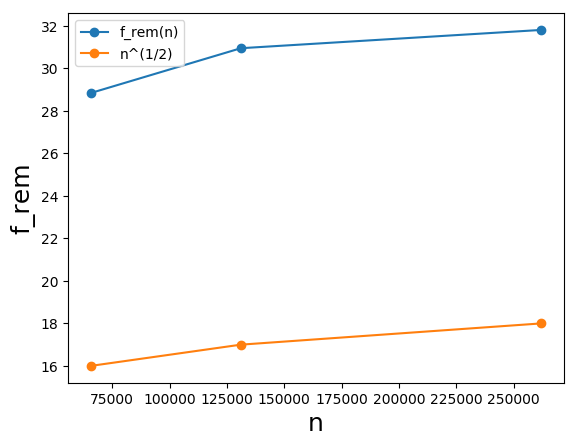
\includegraphics[width=0.95\textwidth]{pictures/med_algo_theo29_rem}
    \end{minipage}
    \hspace*{.3cm}
    \begin{minipage}[t]{.30\textwidth}
        \centering
        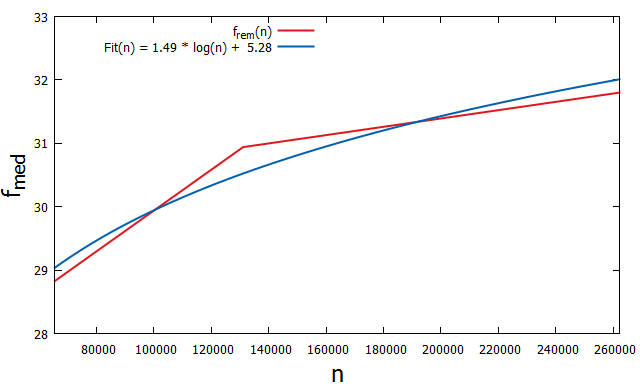
\includegraphics[width=1.25\textwidth]{pictures/med_algo_theo29_fit_rem}
    \end{minipage}
    \hspace*{1.2cm}
    \begin{minipage}[t]{.30\textwidth}
        \centering
        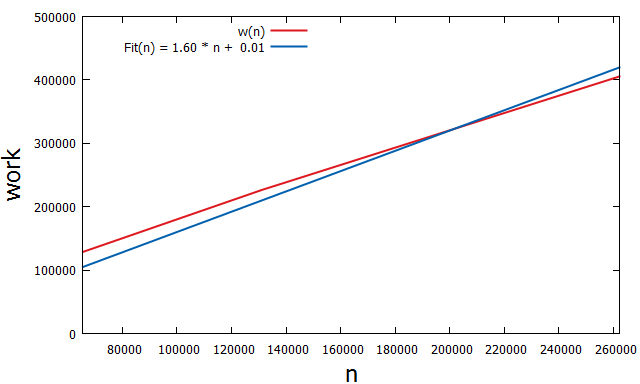
\includegraphics[width=1.25\textwidth]{pictures/med_algo_theo29_fit_work.png}
    \end{minipage}
    \vspace*{-0.1cm}
    \captionof{figure}{Vorhersage und Fit für \fgr sowie die Arbeit $w(n)$.}\label{fig: med_theo29_rem}
\end{figure}

\noindent
Zur Sicherheit wurde die verrichtete Arbeit $w(n)$ noch gegen einen Fit der Form $F(n)= a\cdot n + b$ abgeglichen, der einen nahezu deckungsgleiche Darstellung ergibt.


%---------------------------------------------------------------
\noindent
\newpage

%================================================================
\label{6 : Ausblick}			%	6 : Ausblick	
%----------------------------------------------------------------
%%%%%%%%%%%%%%%%%%%%%%%%%%%%%%%%%%%%%%%%%%%%%%%%%%%%%%%%%%%%%%%%%
\section{Ausblick}		%	AUSBLICK
%%%%%%%%%%%%%%%%%%%%%%%%%%%%%%%%%%%%%%%%%%%%%%%%%%%%%%%%%%%%%%%%%

\noindent
Im Verlaufe dieser Arbeit konnten die in den Theoremen~\ref{theo: min_3}, ~\ref{theo: min_3} und ~\ref{theo: min_3} der Version~\cite{meyer1} aufgestellten Schranken bezüglich der \fg der Elemente des Algorithmus \Rm eindeutig bestärkt werden. Auch wenn weitere Testfälle denkbar wären, so ist die Korrelation zwischen den experimentell gesammelten Daten bereits jetzt unverkennbar.\\[.05cm]
Für den Algorithmus \RM konnte die Linearität der Arbeit $w(n)$ und somit auch Theorem~\ref{theo: med_30} eindeutig bestätigt werden. Für die \fg des Medians sowie aller übrigen Elemente scheinen die Schranken für alle bisher angesammelten Daten eine gute Abschätzung zu liefern, so dass die positive Erwartung besteht, auch die Theoreme~\ref{theo: med_28} und ~\ref{theo: med_29} aus Paper~\cite{meyer2} in naher Zukunft durch weitere Experimentalanalyse weiter stützen zu können.\\[.05cm]
Von weiterem wissenschaftlichen Interesse wäre hier die Entwicklung einer bezüglich ihrer Laufzeit optimierten Implementierung, da die Menge an experimentell gesammelten Daten entscheidend für die Qualität der Analyse ist.\\[.2cm]



%%%%%%%%%%%%%%%%%%%%%%%%%%%%%%%%%%%%%%%%%%%%%%%%%%%%%%%%%%%%%%%%%





\newpage

%================================================================
\label{7 : Data}				%	7 : Data
%----------------------------------------------------------------
%%%%%%%%%%%%%%%%%%%%%%%%%%%%%%%%%%%%%%%%%%%%%%%%%%%%%%%%%%%%%%%%%
\section{Data}		%	DATA
%%%%%%%%%%%%%%%%%%%%%%%%%%%%%%%%%%%%%%%%%%%%%%%%%%%%%%%%%%%%%%%%%

%%%%%%%%%%%%%%%%%%%%%%%%%%%%%%%%%%%%%%%%%%%%%%%%%%%%%%%%%%%%%%%%%
Die Grafiken dieser Arbeit beruhen auf den durch die Implementierung experimentell gewonnen Daten, welche in vollem Umfang bei bei \href{https://github.com/jfklorenz}{Git Hub} eingesehen werden können.\\[.05cm]
Zur Veranschaulichung werden hier die jeweiligen Mittelwerte der experimentellen Daten bezüglich der nach Theorem~\ref{theo: min_5} geforderten Parametrisierung von $k(n)$ aufgeführt.\\[.05cm]
Die tabellarischen Werte entsprechen jeweils dem Mittelwert der Daten aus zehntausend Wiederholungen bezüglich der Auf- und Abrundung des Parameters $k(n)$ sowie der in Kapitel~\ref{other: weigh} diskutierten Gewichtung.

%%%%%%%%%%%%%%%%%%%%%%%%%%%%%%%%%%%%%%%%%%%%%%%%%%%%%%%%%%%%%%%%%
%	DATA - RMINIMUM - Case 2 : log(n) / loglog(n)
%%%%%%%%%%%%%%%%%%%%%%%%%%%%%%%%%%%%%%%%%%%%%%%%%%%%%%%%%%%%%%%%%

\begin{center}
\begin{tabular}{|c|c||c|c|c||c|c|c||c|c|c|}
        	\hline
        	\multicolumn{11}{|c|}{\ccb \textbf{Mittelwerte für $k(n) = \log_2(n) / \log_2\log_2(n)$}}\\
        	\hline
        	\hline
        	\multicolumn{1}{|c|}{\cca \textbf{$\log_2(n)$}}&
        	\multicolumn{1}{c|}{\cca \textbf{$k$}}&
        	\multicolumn{1}{c|}{\cca \textbf{$\lfloor k\rfloor$}}&
        	\multicolumn{1}{c|}{\cca \textbf{\fgm}}&
        	\multicolumn{1}{c|}{\cca \textbf{\fgr}}&
        	\multicolumn{1}{c|}{\cca \textbf{$\lceil k\rceil$}}&
        	\multicolumn{1}{c|}{\cca \textbf{\fgm}}&
        	\multicolumn{1}{c|}{\cca \textbf{\fgr}}&
        	\multicolumn{1}{c|}{\cca \textbf{Ratio}}&
        	\multicolumn{1}{c|}{\cca \textbf{\fgm}}&
        	\multicolumn{1}{c|}{\cca \textbf{\fgr}}\\
        	\hline
        	$6$&$2.32$&$2$& $6.63$&$6.41$ &$3$& $6.50$&$6.32$ &$68-32$&$6.59$ &$6.38$  \\
            \hline
            $7$&$2.49$&$2$&$7.75$ &$7.56$ &$3$& $7.51$ &$7.33$ &$51-49$&$7.61$ &$7.42$  \\
            \hline
            $8$&$2.67$&$2$&$9.11$ &$9.11$ &$3$&$8.84$ &$8.79$ &$33-67$&$8.88$ & $8.84$ \\
            \hline
            $9$&$2.84$&$2$&$10.64$ &$10.56$ &$3$&$10.10$ &$10.03$ &$16-84$&$10.60$ &$10.51$  \\
            \hline
            $10$&$3.01$&$3$&$11.25$ &$11.20$ &$4$&$10.87$ &$11.04$ &$99-1$&$11.12$ &$11.14$  \\
            \hline
            $11$&$3.18$&$3$&$12.65$ &$12.55$ &$4$&$12.05$&$12.50$ &$82-18$&$12.30$ &$12.52$  \\
            \hline
            $12$&$3.35$&$3$&$13.78$ &$13.66$ &$4$&$13.19$&$13.18$  &$65-35$&$13.29$ &$13.26$  \\
            \hline
            $13$&$3.51$&$3$&$15.01$ &$15.04$ &$4$&$14.45$ &$14.95$  &$49-51$&$14.97$ &$15.04$  \\
            \hline
            $14$&$3.68$&$3$&$16.43$ &$16.33$ &$4$& $15.51$ &$15.43$  &$32-68$&$16.15$ &$16.05$  \\
            \hline
            $15$&$3.84$&$3$&$17.53$ &$17.39$ &$4$& $16.75$ &$17.01$  &$16-84$&$17.11$ &$17.19$  \\
            \hline
            $16$&$4$&$4$&$17.89$ &$18.14$ &$4$& $17.89$ &$18.14$  &$any$&$17.89$ &$18.14$  \\
            \hline
            $17$&$4.16$&$4$&$18.36$ &$20.77$ &$5$& $19.03$ &$19.11$  &$84-16$&$18.36$ &$20.77$  \\
            \hline
            $18$&$4.32$&$4$&$19.40$ &$21.04$ &$5$& $20.30$  &$20.83$  &$68-32$&$19.61$ &$20.99$  \\
            \hline
            $19$&$4.47$&$4$&$20.55$ &$22.96$ &$5$&  $21.37$  &$21.30$  &$53-47$&$20.92$ &$22.21$  \\
            \hline
            $20$&$4.63$&$4$&$21.6$ &$23.20$ &$5$&$22.63$  &$23.00$  &$37-63$&$22.30$ &$23.06$  \\
            \hline     
        \end{tabular}\label{Tab: RMin - k=1/2}
        \captionof{table}{Data : \Rm - $k(n) = \log_2(n) / \log_2\log_2(n)$}% Add 'table' caption
\end{center}

%%%%%%%%%%%%%%%%%%%%%%%%%%%%%%%%%%%%%%%%%%%%%%%%%%%%%%%%%%%%%%%%%


























\newpage

%================================================================
\label{8 : Code}				%	8 : Code
%----------------------------------------------------------------
%%%%%%%%%%%%%%%%%%%%%%%%%%%%%%%%%%%%%%%%%%%%%%%%%%%%%%%%%%%%%%%%%
\section{Code}		%	Code
%%%%%%%%%%%%%%%%%%%%%%%%%%%%%%%%%%%%%%%%%%%%%%%%%%%%%%%%%%%%%%%%%
Der in diesem Abschnitt präsentierte Teil des in dieser Arbeit verwendeten Codes soll zur besseren Gesamtverständlichkeit dieser Arbeit beitragen.

\subsection{\Rm}
Anbei die Realisierung der zweiten und dritten Phase des Algorithmus \Rm durch die Methoden \pythoninline{def rmin_phase2} und \pythoninline{def rmin_phase3}.

\subsubsection{Phase 2}
\documentclass[border=3pt]{standalone}
\usepackage{tikz}
\usetikzlibrary{decorations.pathreplacing,patterns}
\definecolor{greengreen}{rgb}{0.0, 0.42, 0.24}
%%%%%%%%%%%%%%%%%%%%%%%%%%%%%%%%%%%%%%%%%%%%%%%%%%%%%%%%%%%%%%%%%
\begin{document}
%%%%%%%%%%%%%%%%%%%%%%%%%%%%%%%%%%%%%%%%%%%%%%%%%%%%%%%%%%%%%%%%%
\begin{tikzpicture}[every node/.style={align=center},
red/.style={fill=red,draw,circle,inner sep=0pt},
blue/.style={fill=blue,draw,circle,inner sep=0pt},
 text width = .35cm]
%================================================================
%	Boxes
\draw[very thick, pattern=north east lines, pattern color=red!20] (-0.5,-0.5) rectangle (20.5,0.5);
\draw[very thick, pattern=north east lines, pattern color=blue!20] (-0.5,1.5) rectangle (20.5,2.5);

%================================================================
%	Nodes
\node[style=red] (r1) at (0,0) {};
\node[style=red] (r2) at (1,0) {};
\node[style=red] (r3) at (2,0) {};
\node[style=red] (r4) at (3,0) {};
\node[style=red] (r5) at (5,0) {};
\node[style=red] (r6) at (6,0) {};
\node[style=red] (r7) at (7,0) {};
\node[style=red] (r8) at (8,0) {};
\node[style=red] (r9) at (12,0) {};
\node[style=red] (r10) at (13,0) {};
\node[style=red] (r11) at (14,0) {};
\node[style=red] (r12) at (15,0) {};
\node[style=red] (r13) at (17,0) {};
\node[style=red] (r14) at (18,0) {};
\node[style=red] (r15) at (19,0) {};
\node[style=red] (r16) at (20,0) {};
%----------------------------------------------------------------
\node (d1) at (0.5,1) {$\vdots$};
\node (d2) at (2.5,1) {$\vdots$};
\node (d3) at (5.5,1) {$\vdots$};
\node (d4) at (7.5,1) {$\vdots$};
\node (d5) at (12.5,1) {$\vdots$};
\node (d6) at (14.5,1) {$\vdots$};
\node (d7) at (17.5,1) {$\vdots$};
\node (d8) at (19.5,1) {$\vdots$};
%----------------------------------------------------------------
\node[style=blue] (b1) at (1.5,2) {};
\node[style=blue] (b2) at (6.5,2) {};
\node[style=blue] (b3) at (13.5,2) {};
\node[style=blue] (b4) at (18.5,2) {};

%================================================================
%	Lines
\draw (r1) -- (d1);
\draw (r2) -- (d1);
\draw (r3) -- (d2);
\draw (r4) -- (d2);
\draw (r5) -- (d3);
\draw (r6) -- (d3);
\draw (r7) -- (d4);
\draw (r8) -- (d4);
\draw (r9) -- (d5);
\draw (r10) -- (d5);
\draw (r11) -- (d6);
\draw (r12) -- (d6);
\draw (r13) -- (d7);
\draw (r14) -- (d7);
\draw (r15) -- (d8);
\draw (r16) -- (d8);
%----------------------------------------------------------------
\draw (d1) -- (b1);
\draw (d2) -- (b1);
\draw (d3) -- (b2);
\draw (d4) -- (b2);
\draw (d5) -- (b3);
\draw (d6) -- (b3);
\draw (d7) -- (b4);
\draw (d8) -- (b4);
%----------------------------------------------------------------
\draw[dashed] (4,3) -- (4,-1);
\draw[dashed] (9,3) -- (9,-1);
\draw[dashed] (11,3) -- (11,-1);
\draw[dashed] (16,3) -- (16,-1);

%================================================================
%	Decoration
\draw[thick, decorate,decoration={brace,amplitude=5pt,mirror}] (0.1,-1.5) -- (2.9,-1.5);
\draw[thick, decorate,decoration={brace,amplitude=5pt,mirror}] (5.1,-1.5) -- (7.9,-1.5);
\draw[thick, decorate,decoration={brace,amplitude=5pt,mirror}] (12.1,-1.5) -- (14.9,-1.5);
\draw[thick, decorate,decoration={brace,amplitude=5pt,mirror}] (17.1,-1.5) -- (19.9,-1.5);

\draw[->, very thick] (10, 1.6) -- (10, 2.4);
\draw[->, very thick] (10, 0.4) -- (10, -0.4);
\node at (9.5,1) {\large $\log_2(k)$};
%----------------------------------------------------------------
\node at (-1,2) {\large $M$};
\node at (-1,0) {\large $L$};
%----------------------------------------------------------------
\node at (1.5,3) {\large $m_1$};
\node at (6.5,3) {\large $m_2$};
\node at (13.5,3) {\large $m_{l/k-1}$};
\node at (18.5,3) {\large $m_{l/k}$};
%----------------------------------------------------------------
\node at (1.5,-1) {\large $L_1$};
\node at (6.5,-1) {\large $L_2$};
\node at (13.5,-1) {\large $L_{l/k-1}$};
\node at (18.5,-1) {\large $L_{l/k}$};
%----------------------------------------------------------------
\node at (1.5,-2) {\large $k$};
\node at (6.5,-2) {\large $k$};
\node at (13.5,-2) {\large $k$};
\node at (18.5,-2) {\large $k$};
%================================================================
\end{tikzpicture}
%%%%%%%%%%%%%%%%%%%%%%%%%%%%%%%%%%%%%%%%%%%%%%%%%%%%%%%%%%%%%%%%%
\end{document}
%%%%%%%%%%%%%%%%%%%%%%%%%%%%%%%%%%%%%%%%%%%%%%%%%%%%%%%%%%%%%%%%%
\subsubsection{Phase 3}
\begin{python}
#   Import
import random

# ==================================================
#   RMinimum: Phase 3
def rmin_phase3(W, k, M, cnt):

    # Generate subsets
    random.shuffle(W)
    W_i = [W[i * k:(i + 1) * k] 
    		for i in range((len(W) + k - 1) // k)]
    W_i_filt = [0 for _ in range(len(W_i))]

    # Filter subsets
    for i in range(len(W_i_filt)):
        W_i_filt[i] = [elem for elem in W_i[i] if elem < M[i]]
        cnt[M[i]] += len(W_i[i])
        for elem in W_i[i]:
            cnt[elem] += 1

    # Merge subsets
    Wnew = [w for sublist in W_i_filt for w in sublist]

    return Wnew, cnt

\end{python}

\newpage
%%%%%%%%%%%%%%%%%%%%%%%%%%%%%%%%%%%%%%%%%%%%%%%%%%%%%%%%%%%%%%%%%
\subsection{\RM}
Anbei die Realisierung der zweiten Phase des Algorithmus \RM durch die Methoden \pythoninline{def rmed_phase3}.
\subsubsection{Phase 2}
\begin{python}
#   Import
import random

# ==================================================
#   RMedian: Phase 2
def rmed_phase2(S, XS, L, C, R, cnt):

    mark = [False for _ in range(len(XS) + len(S))]
    random.shuffle(XS)
    b = len(L)
    
    #	Loop
    for x_i in XS:
        med = 0	#	Check if remaining or discarded
        for j in reversed(range(0, b - 1)):

            current = 2 ** 50	# Arbitrary value
            random.shuffle(L[j])
            for l in L[j]:
                if cnt[l] < current:
                    x_A = l

            if mark[x_A] == True:
                c = 1

            else:
                c = 2

            cnt[x_i] += 1
            cnt[x_A] += 1

            if x_i < x_A:
                if j + c < b:
                    mark[x_i] = True
                    L[j + c].append(x_i)
                    med = -1
                else:
                    med = -2
                break

            current2 = 2 ** 50	# Arbitrary value
            random.shuffle(R[j])
            for r in R[j]:
                if cnt[r] < current2:
                    x_B = r

            if mark[x_B] == True:
                c = 1
            else:
                c = 2

            cnt[x_i] += 1
            cnt[x_B] += 1

            if x_i > x_B:
                if j + c < b:
                    mark[x_i] = True
                    R[j + c].append(x_i)
                    med = 1
                else:
                    med = 2
                break
        
        #	Sort remaining elements in C 
        # 	and discarded in the outer buckets.
        if med == 0:
            C.append(x_i)
        elif med == -2:
            L[len(L) - 1].append(x_i)
        elif med == 2:
            R[len(R) - 1].append(x_i)
    
    return S, XS, L, C, R, cnt
\end{python}

\newpage
%%%%%%%%%%%%%%%%%%%%%%%%%%%%%%%%%%%%%%%%%%%%%%%%%%%%%%%%%%%%%%%%%
\subsection{Werkzeug}
Neben den Algorithmen wurden weitere Werkzeuge zur Datenverarbeitung implementiert.\\[.05cm]
Anbei beispielhaft das \textit{Bash}-Skript, welches genutzt wurde, um mit dem \textit{Goethe-HLR} Cluster zu kommunizieren, sowie eine \textit{Gnuplot}-Datei~\cite{gnu} zur Berechnung eines Fits mithilfe des \textit{Marquardt-Levenberg} Algorithmus~\cite{gnu2}. 
\subsubsection{Server}
\textit{Bash}-Skript zur Ausführung der Datei \textit{python\_py1.py} auf dem \textit{Goethe-HLR} Cluster.
\begin{lstlisting}[style=bsh]
#!/bin/bash
#SBATCH --partition=general1
#SBATCH --nodes=1
#SBATCH --ntasks=40
#SBATCH --cpus-per-task=1
#SBATCH --mem=100000
#SBATCH --time=10:00:00
#SBATCH --mail-type=FAIL

export OMP_NUM_THREADS=1
export PYTHONHOME=/home/memhierarchy/lorenz/venv
export PYTHONPATH=/home/memhierarchy/lorenz/venv/python

# Run 10 times
/home/memhierarchy/lorenz/venv/bin/python py1.py >& 01.out &
...
/home/memhierarchy/lorenz/venv/bin/python py1.py >& 01.out &

# Wait for all child processes to terminate.
wait
\end{lstlisting}
\subsubsection{Fit}
\textit{Gnuplot}-Skript zur Berechnung eines Fits bezüglich der Daten aus der Datei \textit{filename.csv} und der Funktion $f(x)=a\cdot \log_2(x)/\log_2\log_2(x) + b$ mit Startwerten $a=6.5$ sowie $b=-8.5$.
\begin{lstlisting}[style=gnu]
#	General
set datafile separator ",";

#	Beschriftung
#set title 'Fit : f(n) = a * eps^(-1) * log2log2(n) + b' font ",18"
set key autotitle columnhead
set xlabel 'n' font ",18"
set ylabel 'f_{min}' font ",18"
set key left top

#	Ranges
set logscale x
set xrange[64:1048576]
set yrange[0:30]

#	Style
set style line 1 \
    linecolor rgb '#0060ad' \
    linetype 1 linewidth 2 \
    pointtype 7 pointsize 1.5

set style line 2 \
    linecolor rgb '#dd181f' \
    linetype 1 linewidth 2 \
    pointtype 5 pointsize 0.5

#	Fit Parameters
FIT_LIMIT=1e-6;
a=6.5; b=-8.5

#	Fitting Function:
f(x) = a * log(x, 2) / log(log(x ,2) , 2) + b
fit f(x) "filename" u 1:2 via a,b

#	Plot
set logscale x 2
ti = sprintf("F(n) = %.2f * log2(n)/log2(log2(n)) +  %.2f", a, b)
plot "filename.csv" using 1:2 with lines ls 2, \
	f(x) t ti with lines ls 1

#	Output
set term png size 800,800;
\end{lstlisting}

\newpage
%================================================================

\label{0 : Literatur}			%	0: Literaturverzeichnis
%----------------------------------------------------------------
%%%%%%%%%%%%%%%%%%%%%%%%%%%%%%%%%%%%%%%%%%%%%%%%%%%%%%%%%%%%%%%%%
\label{Bibliography}	%	BIBLIOGRAPHY
%%%%%%%%%%%%%%%%%%%%%%%%%%%%%%%%%%%%%%%%%%%%%%%%%%%%%%%%%%%%%%%%%
\begin{thebibliography}{9}
%----------------------------------------------------------------
\bibitem{meyer1}
  \textit{Fragile complexity of some classic comparison based problems}, 
  Afshani, Peyman and Fagerberg, Rolf and Hammer, David and Jacob, Riko and Kostitsyna, Irina and Meyer, Ulrich and Penschuck, Manuel and Sitchinava, Nodari, 
  Institute for Computer Science, J. W. Goethe University, 60325 Frankfurt/Main, Germany, 2018 - 06 - 14
%----------------------------------------------------------------

\bibitem{meyer2}
  \textit{Fragile complexity of some classic comparison based problems}, Afshani, Peyman and Fagerberg, Rolf and Hammer, David and Jacob, Riko and Kostitsyna, Irina and Meyer, Ulrich and Penschuck, Manuel and Sitchinava, Nodari, 
  Institute for Computer Science, J. W. Goethe University, 60325 Frankfurt/Main, Germany, 2019 - 01 - 09

%----------------------------------------------------------------
\bibitem{chaud}
	\textit{Probabilistic recurrence relations revisited}, Shiva Chaudhuri, Devdatt Dubhashi,
	Theoretical computer science, Elsvier, 1997

%----------------------------------------------------------------
\bibitem{gnu}
	\textit{gnuplot 5.2, An Interactive Plotting Program}, Thomas Williams \& Colin Kelley, Gnuplot Documentation. \newline Link: \url{http://www.gnuplot.info/docs_5.2/Gnuplot_5.2.pdf}

\bibitem{gnu2}
	\textit{Optimierung und inverse Probleme}, Prof. Dr. Bastian von Harrach, Goethe-Universität Frankfurt am Main
Institut für Mathematik, Wintersemester 2016/17

\bibitem{aks}
	\textit{V. Chv´atal. Lecture notes on the new AKS sorting network},  Technical Report DCS-TR-294, Department of Computer Science, Rutgers University, New Brunswick, NJ, 1992, October
	
	




  
\end{thebibliography}
%%%%%%%%%%%%%%%%%%%%%%%%%%%%%%%%%%%%%%%%%%%%%%%%%%%%%%%%%%%%%%%%%
\newpage

\listoffigures
\newpage

\listoftables
\newpage

\section*{Danksagung}
\addcontentsline{toc}{section}{Danksagung} 
\noindent
Hiermit möchte ich mich in aller Form bei meiner Familie für all die Liebe und konstruktive Kritik, meinen Freunden für ihre aufbauenden Worte und den Stress vergessenden Abenden, meiner Freundin für all die aufrichtige Fürsorge und meinen Kommilitonen und Kollegen für ihre anregenden Gedanken und messerscharfen Blick beim Auffinden meiner Fehler danken.

\noindent
Ohne euch wären diese Zeilen nie geschrieben worden. Ich danke euch allen aus tiefstem Herzen.
%%%%%%%%%%%%%%%%%%%%%%%%%%%%%%%%%%%%%%%%%%%%%%%%%%%%%%%%%%%%%%%%%
\label{End Document}
\end{document}
%%%%%%%%%%%%%%%%%%%%%%%%%%%%%%%%%%%%%%%%%%%%%%%%%%%%%%%%%%%%%%%%%
